
\documentclass[a4paper,12pt]{article}

\usepackage{amsmath,amssymb,amsfonts,amsthm}    % Typical maths resource packages
\usepackage{graphicx}                           % Packages to allow inclusion of graphics
\usepackage{hyperref}                           % For creating hyperlinks in cross references
\usepackage[authoryear]{natbib}                 % literature reference style
\usepackage[bf]{caption2}

%For float barriers include placeins
\usepackage{placeins}

%To enable different margins on the title page
\usepackage[paper=a4paper,margin=2cm]{geometry}


% -------------------------------
% --- some layout definitions ---
% -------------------------------

% define topline
\usepackage[automark]{scrpage2}
\pagestyle{scrheadings}
\automark{section}
\clearscrheadings
\ohead{\headmark}

% define citation style
\bibliographystyle{ecta}

% define line line spacing = 1.5
\renewcommand{\baselinestretch}{1.5}

% define second level for `itemizing'
\renewcommand{\labelitemii}{-}




% --------------------------------------
% --------------------------------------
% --------------------------------------
% --- the structure the tex document ---
% ---  (this our recommendation) -------
% frontmatter:
%   - titlepage (mandatory),
%   - acknowledgement,
%   - abstract,
%   - table of contents (mandatory),
%   - list of abbreviations (not mandatory),
%   - list of figures (not mandatory),
%   - list of tables  (not mandatory) .
%
% body of the thesis (the structure of the thesis body is not mandatory, but the list of literature is mandatory):
%   - introduction,
%   - methods,
%   - data,
%   - results,
%   - conclusion,
%   - literature (mandatory),
%   - appendix (figures, tables).
%
% last page:
%   - declaration of authorship (mandatory).
% --------------------------------------
% --------------------------------------
% --------------------------------------

\begin{document}

% -------------------------------
% --- frontmatter: Title page ---
% -------------------------------

\thispagestyle{empty}
\begin{center}

    {\Large{\bf The effects of Education and individual Labor Market History in the GDR on Labor
Market performance after Reunification: An empirical Analysis based on the BIBB-IAB
Survey 1991/92 or the GSOEP}} \vspace{0.5cm}


    {\normalsize Seminar Paper submitted\\\vspace{0.5cm}
    to}\\\vspace{0.5cm}
    {\normalsize{\bf Prof. Ph.D. Bernd Fitzenberger}} \\\vspace{0.5cm}
    {\normalsize Humboldt-Universit\"at zu Berlin \\
    School of Business and Economics \\
    Institute for Statistics and Econometrics \\
    Chair of Econometrics} \vspace{1cm}


    {\normalsize by \\\vspace{0.5cm}
    {\bf Christian Koopmann} \\
   572485} \vspace{1cm}


    {\normalsize completed in the course of the seminar \\
    {\bf Econometric Projects WS 16/17} \\
    Berlin, February 13, 2017}

\end{center}




% ------------------------------------
% --- frontmatter: Acknowledgement ---
% ------------------------------------
\newpage
\newgeometry{top=2.5cm,bottom=2.5cm,right=1.5cm,left=4cm}
\pagestyle{plain}
\pagenumbering{roman}   % define page number in roman style
\setcounter{page}{1}    % start page numbering






% -----------------------------
% --- frontmatter: Contents ---
% -----------------------------
\newpage
\tableofcontents
\clearpage


% ----------------------------------------------------
% --- frontmatter: List of Figures (not mandatory) ---
% ----------------------------------------------------
\newpage
\addcontentsline{toc}{section}{List of Abbreviations}
\ohead[]{LIST OF ABBREVIATIONS}
\section*{List of Abbreviations}

\begin{tabular}{rp{0.2cm}lp{1cm}}
    BIBB    & &  Bundesinstitut für Berufsbildung \\
    CPI     & &  Consumer Price Indes  \\
    FRG     & &  Federal Republic of Germany \\
    GDR    & &  German Democratic Republic \\
    GSOEP & & German Socio Economic Panel\\
    IAB & & Institut für Arbeitsmarkt- und Berufsforschung \\
    OLS & & Ordinary Least Squares\\
    POLS & & Pooled Ordinary Least Squares
\end{tabular}




% ----------------------------------------------------
% --- frontmatter: List of Figures (not mandatory) ---
% ----------------------------------------------------
\newpage
\addcontentsline{toc}{section}{List of Figures}
\ohead[]{\rightmark}
\listoffigures



% ---------------------------------------------------
% --- frontmatter: List of Tables (not mandatory) ---
% ---------------------------------------------------
\newpage
\addcontentsline{toc}{section}{List of Tables}
\listoftables



% -------------------------------
% --- main body of the thesis ---
% -------------------------------
\newpage
\pagestyle{plain}
\setcounter{page}{1}    % start page numbering anew
\pagenumbering{arabic}  % page numbers in arabic style


\section{Introduction} \label{Sec:Intro}
\subsection{Motivation}
From the perspective of an labour economist the transition of countries from planned to market based economies in the early nineteen-nineties offers both a variety of interesting research questions with high policy relevance as well as the chance to evaluate the validity of various assumptions regarding labour markets.
The abruptness of the political change and the existence of a benchmark economy with the same institutional framework let the territory of the former German Democratic Republic stand out among other transitional economies in Europe. These aspects also enable analytical approaches that are not applicable in any other transitional economy.
The economical as well as the political importance of a successful integration of East Germany into the Economy of the Federal Republic generates many research problems with high policy relevance. This is especially true for the area of labour economics since differences in the wage levels as well as unemployment rate are often one of the main sources of public discontent regarding the economic development of East Germany. Persisting differences in both of these measures between East and West Germany show, that these topics remain relevant even a quarter of a century after reunification.  
\subsection{Problem Definition}
The original problem was researching the effect of pre-unification Education and Labor Market History in the GDR on the performance in the post-unification Labor Market. Based on the intention to analyse the dynamics of labour markets on a longer time frame including more recent data the decision was made to limit the focus on research questions that could be analysed using the data from the German Socio Economic Panel (GSOEP). Although this is a very rich panel dataset it includes less detailed information regarding the contents of employment than the BIBB-IAB survey mentioned in the title. From this decision it was therefore clear that the Labor Market History in the GDR would be mainly captured by the amount of experience gathered pre unification. Inspired by (\cite{gathmann_understanding_2004}) the focus was narrowed down to analyse the changing returns to education and experience from 1991 to 2014. Regarding this three research questions emerged to guide the analysis:

\begin{enumerate}
		\item \textit{How do returns to education and experience differ in East and West Germany ?} 
	\item \textit{How do these differences develop over time ?}
	\item \textit{How do these differences behave when differentiating between Experience and Education obtained pre- / post-unification?}
\end{enumerate}

Originally these questions were also analysed separately for different age and skill groups. However in the interest of brevity and clarity these aspects were not included in this report. 


\subsection{Literature Overview}
The uniqueness of the East German Labour market described above as well as the availability of high quality datasets have sparked a significant amount of research and publication on the German Labour market during the transition. A lot of these studies also make use of the GSOEP data.
Especially the first two the research questions have been the focus of many scientific papers in this area, most of which however are focused on the returns to experience. These studies have shown much flatter wage profiles across age  (\cite{krueger_comparative_1992},\cite{burda_getting_1997}) as well as experience (\cite{jurajda_when_2007}) in East Germany both before and in the first years after reunification, although the East German wage structure has changed significantly in the first years after reunification to resemble the West German structure more closely. (\cite{krueger_comparative_1992} shows that some of these differences especially regarding the experience profile persist for employees migrating from East to West Germany.
One study concludes that "... ,while endowments of education and training are comparable if not favourable in the East, returns to age were depressed under socialism and continue to be so several years after market relations were introduced."(\cite{burda_getting_1997}
, p. 24) suggesting very different findings regarding these research questions for experience and education. It has been shown that even after extending the analysis well into the twenty-first century and applying non-OLS estimators to account for endogeneity some of these differences persist (\cite{orlowski_east_2009}).
As mentioned above the main inspiration in the design of this study has been (\cite{gathmann_understanding_2004}), where Experience is separated into those years of experience gathered before reunification and those gathered after. In this paper it is found "... that socialist labor market experience has lost its economic value in the post-unification
labor market"(\cite{gathmann_understanding_2004}, p. 13).
One might summarise some of these results using the following hypotheses Regarding each of the research questions posed above:

\begin{enumerate}
	\item Returns to Education are similar in the East and West whereas returns to experience differ more widely. 
	\item Whereas returns show signs of convergence between East and West in the early years after reunification this trend slows and significant differences remain even decades later.
	\item Experience gathered in the GDR is of no value in the post reunification labour market.
\end{enumerate}

In Addition to testing these hypotheses this study will extend the literature in several ways. First of all the analysis will be extended to the whole time frame post reunification for which the GSOEP data is available (1991 - 2014). Instead of the binary comparison between pre- and post reunification which is the focus of most papers (especially early ones) this study will therefore be focused on the dynamic behaviour of wage structures post reunification. The approach of differentiating between New and Old Experience (\cite{gathmann_understanding_2004}) will be extended to Education and also applied to West German data to enable relative comparison. 



\section{Methodology}\label{Sec:Method}
\subsection{Approach}
To estimate the returns to education and experience in East and West Germany as well as their changes over time the following approach will be applied:
\begin{enumerate}
	\item Wherever possible the variables New and Old Experience or Education are generated from the total levels of Experience and Education (see Section \ref{Sec:Data}). All observations for which this is not possible will be dropped from dataset.
	\item The data is separated into separate sub samples according to Region (East / West) as well as survey year (periods of four years from 1991 - 2014).
	\item The two models described below are estimated separately on each of the twelve  sub samples using pooled OLS.
	\item Statistics of interest are calculated for each of the sub samples (see Section \ref{Sec:Results}).	
\end{enumerate}

  
\subsection{Models}
In step two of the approach described above the following two models are fitted to the data:
\begin{equation}
	\begin{split}
	log(Wage) &= \beta_{1}TotalEdu + \beta_{2}TotalExp + \beta_{3} TotalExp^2\\
	&+\beta_{4}Tenure + \beta_{5}YearDummie + \beta_{6}Sex
	\end{split}
\end{equation}
\begin{equation} 
	\begin{split}
	log(Wage) &= \beta_{1a}OldEdu + \beta_{1b}NewEdu + \beta_{2a}OldExp \\
	&+ \beta_{2b}NewExp + \beta_{3a}OldExp^2 + \beta_{3b}NewExp^2\\
	&+\beta_{4}Tenure + \beta_{5}YearDummie + \beta_{6}Sex
	\end{split}
\end{equation}
All following results regarding Total Education and Experience are therefore based on the first model whereas all results regarding New and Old Experience or Education are based on the second one.
In the following a short definition/explanation will be given for each variable:

\begin{description}
	\item[Wage] Gross monthly wage deflated to 2010 price levels. This is the variable \textit{pglabgro} from the \textit{SoepLong pgen} dataset. 
	\item[TotalEdu] Total years of education gained both pre and post-reunification. This is the variable \textit{pgbilzt} from the \textit{SoepLong pgen} dataset. This variable is generated based on the type of degrees the individual obtained and is set to its minimum value 7 when no degree was obtained.
	\item[TotalExp] Total years of full time experience gained both pre- and post-reunification. This is the variable \textit{pexpft} from the \textit{SoepLong pgen} dataset.
	\item[Old Edu] Amount of Total Education gained before reunification. For most individuals this is set to the level of Total Education they had in 1990. For some younger individuals in later samples this is generated on the assumption that they started their education at age 6 and finished it consecutively.
	\item[Old Exp] Amount of Total Experience gained before reunification. For most individuals this is set to the level of Total Education they had in 1990. For some younger individuals in later samples this is set to zero if they have finished their education after reunification.
	\item[YearDummie] These are actually several dummie variables for each year in one period except the first, which is the reference year.
	\item[Tenure] Time spent with current employer (across different positions) in years. This is the variable \textit{pgerwzt} from the \textit{SoepLong pgen} dataset.
	\item[Sex] Dummie variable indicating whether an individual is female. 
	 
	
\end{description}

\newpage
\section{Data and Descriptive Evidence} \label{Sec:Data}
The data used in this analysis consists of the data on all full time employed individuals in the A and C samples of the Socio Economic Panel. To slow the ageing and attrition of the sample individuals from later samples were also included when the amount of Old and New Experience or education could still be inferred with reasonable accuracy. These include mainly younger individuals for whom education was finished after reunification and therefore all experience can be assumed to be New experience. In this section first the distribution of gross monthly wages are analysed in East and West Germany across different groups regarding experience and education. This will give some first insights hypothesises regarding the research questions stated above. Afterwards the distribution of these explanatory variables themselves will be analysed, which will be helpful in understanding and interpreting the results in Section \ref{Sec:Results}.
\subsection{Distribution of Wages}
Regarding the overall mean wages in  the East and West German sample one can observe from Figure \ref{fig:MeanWages} that wage levels in the East  started off at a much lower level than in the West. Whereas in the early nineties there was a substantial increase in East German wages relative to the West, this convergence has slowed and there remains a sizeable difference even in the last time period. 
With respect to the distribution of wages across total experience Figure \ref{fig:MeanWagesByTotalExp} shows a similar picture. The wage distribution across overall experience started out very flat in East Germany but then converged towards a similar relative wage structure as in the West over time. This convergence appears at a much higher rate in the nineties and has since slowed down sharply. From this analysis one might expect to see relative returns to total education start off from a significantly lower level the west with regional differences decreasing rapidly in the nineties but then remaining at still somewhat lower levels in later years.
In Figures \ref{fig:MeanWagesByOldExp} and \ref{fig:MeanWagesByNewExp} this analysis is repeated separately for Old and New Experience. Here we see a striking differences between the two kinds of experience. Throughout the time frame there is virtually no difference in mean wages across Old Experience in East Germany. This suggests that experience gathered in the GDR has no effect on the wages post reunification. When comparing this with the picture for West Germany where there are large differences across Old Experience in the early years after reunification, which then disappear over time, this implies, that this difference is probably due to the low quality of human capital obtained through work experience gathered in the socialist economy. Regarding the wage profile across new experience one is faced with the problem that the amount of New Experience an individual has in any given year is limited by the time that has passed since reunification. Therefore early after reunification there are no individuals individuals in the upper groups and the analysis based on Figure \ref{fig:MeanWagesByNewExp} is limited to later years. Although it is not immediately obvious from looking at the graph, the relative differences between the groups is higher in the West throughout the 2000s, a difference that is decreasing only sightly over time.
Regarding the wage profile across education one can see from Figure \ref{fig:MeanWagesByTotalEdu} that education has some effect in East Germany immediately after reunification, which is much lower than in the West. Throughout the whole time frame however the relative wages of the highest education group in East Germany rise steadily and the regional wage distributions seem relatively similar at the end of the time frame. In Figure \ref{fig:MeanWagesByOldEdu} we see an overall relatively similar picture for Old Education which suggests, that the above observations regarding the obsolescence of Old Experience do not apply to education.

\subsection{Distribution of Explanatory Variables}
To better understand and interpret the results in section \ref{Sec:Results} it is useful to take a look at the different regional levels of Experience and Education over time. 
From Figure \ref{fig:MeanExp} one can see that the total level of experience is higher in the West than it is in the East, with the relative difference being particularly high with regards to Old Experience. With respect to education one can see from Figure \ref{fig:MeanEdu}, that while the total levels of education are relatively similar in both regions, people in the East tend to have a higher share of Old Education. Both of these observations can be explained by an overall higher mean age of the East German sample.



\FloatBarrier
\newpage
\section{Results} \label{Sec:Results}
In the following paragraphs, the results obtained through the modelling approach specified in Section \ref{Sec:Method} will be illustrated in a mostly graphical way.
Due to the non-linearity of the experience term in the models specified above the effect of experience on wages would not be immediately obvious from the coefficients. Therefore the returns to experience will be captured through the predicted contribution of 5 years of experience to the log wage. To get this contribution for Total Experience in West Germany in the time period from 1991 to 1994 for example one would calculate: 
	\begin{equation} 
	Diff_{0-5,TotalExp}^{(9194, West)} = \hat{\beta}_{2}^{(9194, West)}*5 + \hat{\beta}_{3}^{(9194, West)} * 5^2
	\end{equation}

In this case $\hat{\beta}_{2}^{(9194, West)}$ would be the estimate for $
\beta_{2}$ from the first model specified in Section \ref{Sec:Method} using Pooled OLS on the sub sample of observations with survey years between 1991-1994 and sample region West Germany. This statistic  will be called \textit{Returns to Total Experience} henceforth. The values for New and Old Experience are calculated in an analogous way based on the Coefficients of the second model. Although education enters the wage regression only linearly and its effect could therefore be evaluated directly from the coefficients, it is evaluated in the same way as experience for the sake of simplicity and comparability. 
As seen in Section \ref{Sec:Data} however the sub samples differ significantly regarding the mean levels of each of the explanatory variable. On the one hand this will significantly affect the estimated returns as specified above, on the other it also makes it harder to judge the amount of human capital that is stored in each kind of experience and education for each of the sub samples. Therefore in the following results another statistic has been calculated, which can be explained as the mean value of the predicted contribution of each variable to the log wage. In the case of Total Experience and for the same sub sample as before this would be calculated as follows, where $I_{9194}^{west}$ is the set of all observations in that subset and $|I_{9194}^{west}|$ is the total number of those observations:
	\begin{equation} 
	\begin{split}
	Diff_{TotalExp}^{(9194, west)} =& \frac{1}{|I_{9194}^{west}|}\sum_{i \in 	I_{91-94}^{west}} \hat{\beta}_{2}^{(9194, west)}*TotalExp_{i}\\
 	&+\hat{\beta}_{3}^{(9194, west)} * TotalExp_{i}^2
	\end{split}
	\end{equation}
This value is then called \textit{Average Human Capital in Total Experience} in West Germany during the period of 1991 - 1994. Again the values for the other explanatory variables would be calculated analogously. 
\subsection{Experience}
From Figure \ref{fig:DiffComparisonExp} one can draw several observations regarding the development of returns to experience for the different sample regions. First of all and most obviously one can see that the returns for all types of experience in the West constantly exceed those in the East. Also the results seem to confirm the hypothesis regarding Old Experience gained from the Literature and the Analysis in Section \ref{Sec:Data}, namely that Old Experience is of no positive value in East Germany, but starts off with positive value in the West which then converges towards zero. Also can observe that the returns to New Experience converge toward those of Total Experience for both sample regions. As one might have expected the returns to Total Experience lie somewhere between those of New and Old Experience for each of the sub samples.
Based on the results in Figure \ref{fig:HumanCapitalExp} one can see that the trends observed for the returns to Old Experience are even more clearly visible regarding the Human Capital in Old Experience which is quite high for West Germany immediately after reunification but then converges towards zero. Due to the declining amount of Old Experience present in the sample the fluctuations and negative values observed for the returns in the later periods are somewhat smoothed and less visible with regard to human capital.
However regarding New Experience the rising amount of this kind of experience in the samples more than compensates the falling returns observed above and lead to slightly rising trend of Human Capital stored in New Experience. On the first glance it might be surprising that the amount of human capital stored in New Experience exceeds the value for total experience, however it is important to keep in mind that these are based on two different models and although $TotalExp = NewExp + OldExp$ holds, the same cannot be said for the estimated returns and human capital values. One might also observe from this graph that the relative Human Capital stored in New Experience for West Germans exceeds that for their East German counterparts by a relative constant margin, even though the amount of New Experience is actually higher in the East German sample in later periods.



\subsection{Education}
From Figure \ref{fig:DiffComparisonEdu} we can see that the differences in returns between different kinds of education and sample regions are much smaller than in the case of experience. One can see a steep increase in the returns to New Education, however one should bare in mind that there is virtually no New Education in the earlier sub samples. When looking at later periods where mean levels of the different kind of education are relatively similar one can see very similar values for Old, New and Total Education. This suggests that there is no notable difference in the value of Old and New Education in either of the sample regions. One can also see a rising trend in the returns to all types of education. This trend is steeper in East Germany leading to East German relative returns to education exceeding those in the West in the later samples. Regarding the relative Human Capital stored in the different types of Education one can see in Figure \ref{fig:HumanCapitalEdu} a positive trend for Total Education throughout the time frame, again at a steeper rate in the East than in the West resulting in higher levels in the East for later Periods. Regarding the different types of Education one can see not surprisingly a steeply rising share of human capital  in New Education a trend more pronounced in the West German sample where the human capital in New Education is higher throughout the time frame. 


\newpage
\section{Conclusions}\label{Sec:Conc}
In the following paragraphs the results of this study will be summarized with regards to the research questions defined in section \ref{Sec:Intro} and the policy implications of these results discussed. Also an outlook will be given into possible ways to extend the research in this study especially with regards to limitations of this study.
\subsection{Research Questions}
Concerning the research questions posed above this study comes to the following conclusions:
\subparagraph*{How do returns to education and experience differ in East and West Germany ?} Overall the differences in relative returns to education are quite small across sampling regions. This also holds when looking at the relative human capital stored in education, which is in fact higher in the East for later periods.  For relative returns to and human capital stored in experience a somewhat different picture emerges. Both are significantly lower in the East throughout the time frame despite higher overall levels of experience in the East German samples.
\subparagraph*{How do these differences develop over time ?}
	Especially regarding the returns to experience there has been a period of rapid decrease in the nineteen-nineties. This trend however has significantly slowed since and there remains a sizeable regional gap relative returns and human capital even 24 years after reunification which shows no trend of disappearing.  
\subparagraph*{How do these differences behave when differentiating between Experience and Education obtained pre- / post-unification?}
	This study was able to confirm the results regarding Experience gathered in the German Democratic Republic from the literature as well as the observations regarding this topic from the exploratory data analysis. This type of experience seems to have no positive effect on wages in the post reunification labour market, and can therefore be said to be obsolete in some sense. In extension to the existing literature this result has been made even clearer when comparing the results to those for experience gathered in the Federal Republic pre unification which does retain value in the first decade after reunification. Therefore this relative lack of returns to Old Experience can not be simply explained by the time passed since reunification but is most likely caused by an inferior quality of work experience gathered under socialism. This fact also offers a possible  explanation for the rapid decreases of differences in the returns to experience in the nineteen-nineties. During this time initially rather high returns to Old Experience in West Germany converged towards zero slowly eliminating this source of regional differences in the wage profile. However the since remaining difference in returns to experience seems to be the part caused by the persisting  difference in evaluations of work experience gathered since reunification. Regarding Education there seems to be no difference between the pre- and post unification and regional differences seem to be rather low for all types and all time periods. 
\subsection{Policy Implications}
The results of this study have implications regarding both the evaluation of past policies pursued since reunification and the design and selection of new policies aimed at reducing economic imbalances between East and West Germany. First it offers a more precise evaluation of policies aimed at providing work experience for struggling workers in East Germany. Some studies have cited the flat wage distribution across experience as evidence against these kind of policies. However since these policies would increase the amount of New Experience, which provides much higher returns, this study offers a more positive view on these kind of policies. Since old individuals have a higher share of work experience gathered pre unification this study also provides evidence that these individuals are especially vulnerable to relative wage losses and might be chosen as the target group of policies mitigating these effects. Another group of individuals especially vulnerable to erosion of human capital are those individuals which have lower levels of education and a higher share of human capital in generally experience, since these people will not profit from the high returns to education in East Germany. Again this group might be of special interest in policy design. Another effect of these high returns to education might be favouring policies that aim at enabling workers in East Germany to update their education levels as opposed to those that aim to provide work experience.
\subsection{Limitations / Future Research}
One of the main Limitations in this study with regards to the interpretation of the results, might be the fact that it offers no insight into wether differences in returns are due to different evaluations of the same human capital in East and West Germany or whether it is due to differences in quality of experience or education gathered in each of the regions. One way to get some insight into this might be analysing the labour market performance of migrants who have gained their experience in one region but earn their wage in the other region. Whether this is possible with the GSOEP data however is questionable since it contains relatively few migrants. Another aspect to consider are different price levels in East and West Germany, for which this study does not account. Adjusting wages to purchasing parity levels might give somewhat different results, which might be more relevant when analysing the economic situation of individuals in East Germany. Another area in which one might be able to improve upon this study is methodology. Since models are fitted on to time periods of several years, each of these estimations is still done on panel data. Regarding the limitations of Pooled OLS in this case and the possibility to apply different estimation methods, further research might be of relevance. Another direction of further research could also be analysing how the results to above questions differ with individuals of different characteristics. In the progress of this study this has been done among others for people with different degrees and has shown some promise.



% ----------------
% --- appendix ---
% ----------------
\appendix

% literature
\newpage
\addcontentsline{toc}{section}{References}
\bibliography{literature}

% figures (not mandatory)
\newpage
\section{Figures}

 
\begin{figure}[!h]
    \centering
    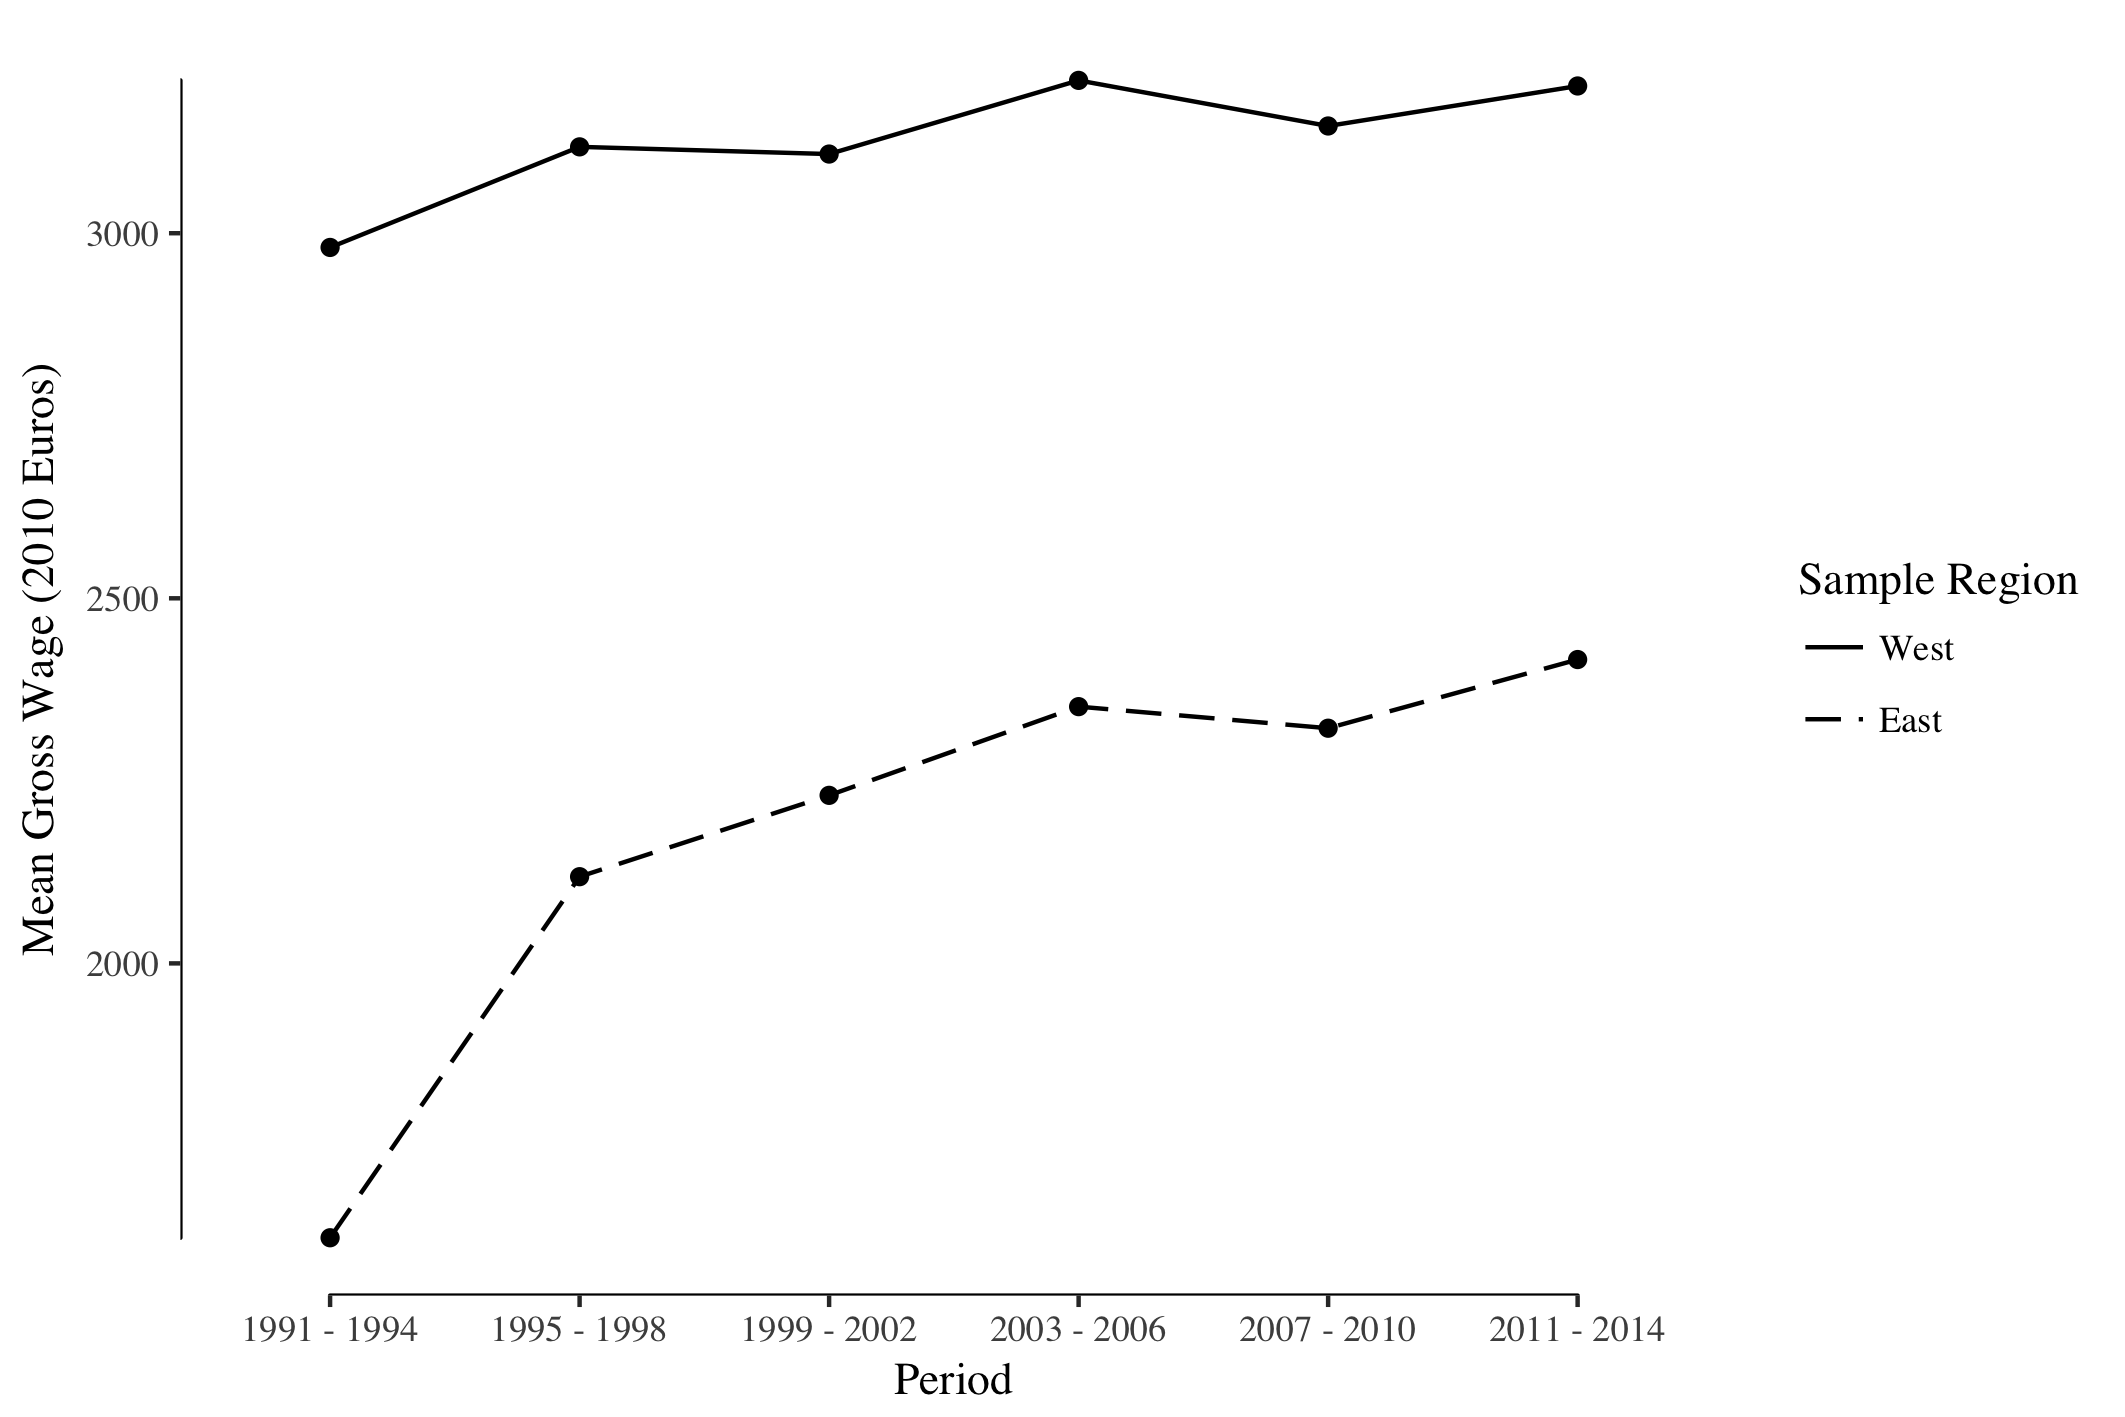
\includegraphics[width=\textwidth]{/Users/Christian/Statistik_Studium/EconProject/Code/Graphics/plotMeanWages.png}
    \caption{Average Wages}
    \label{fig:MeanWages}
\end{figure}

\begin{figure}[!h]
    \centering
    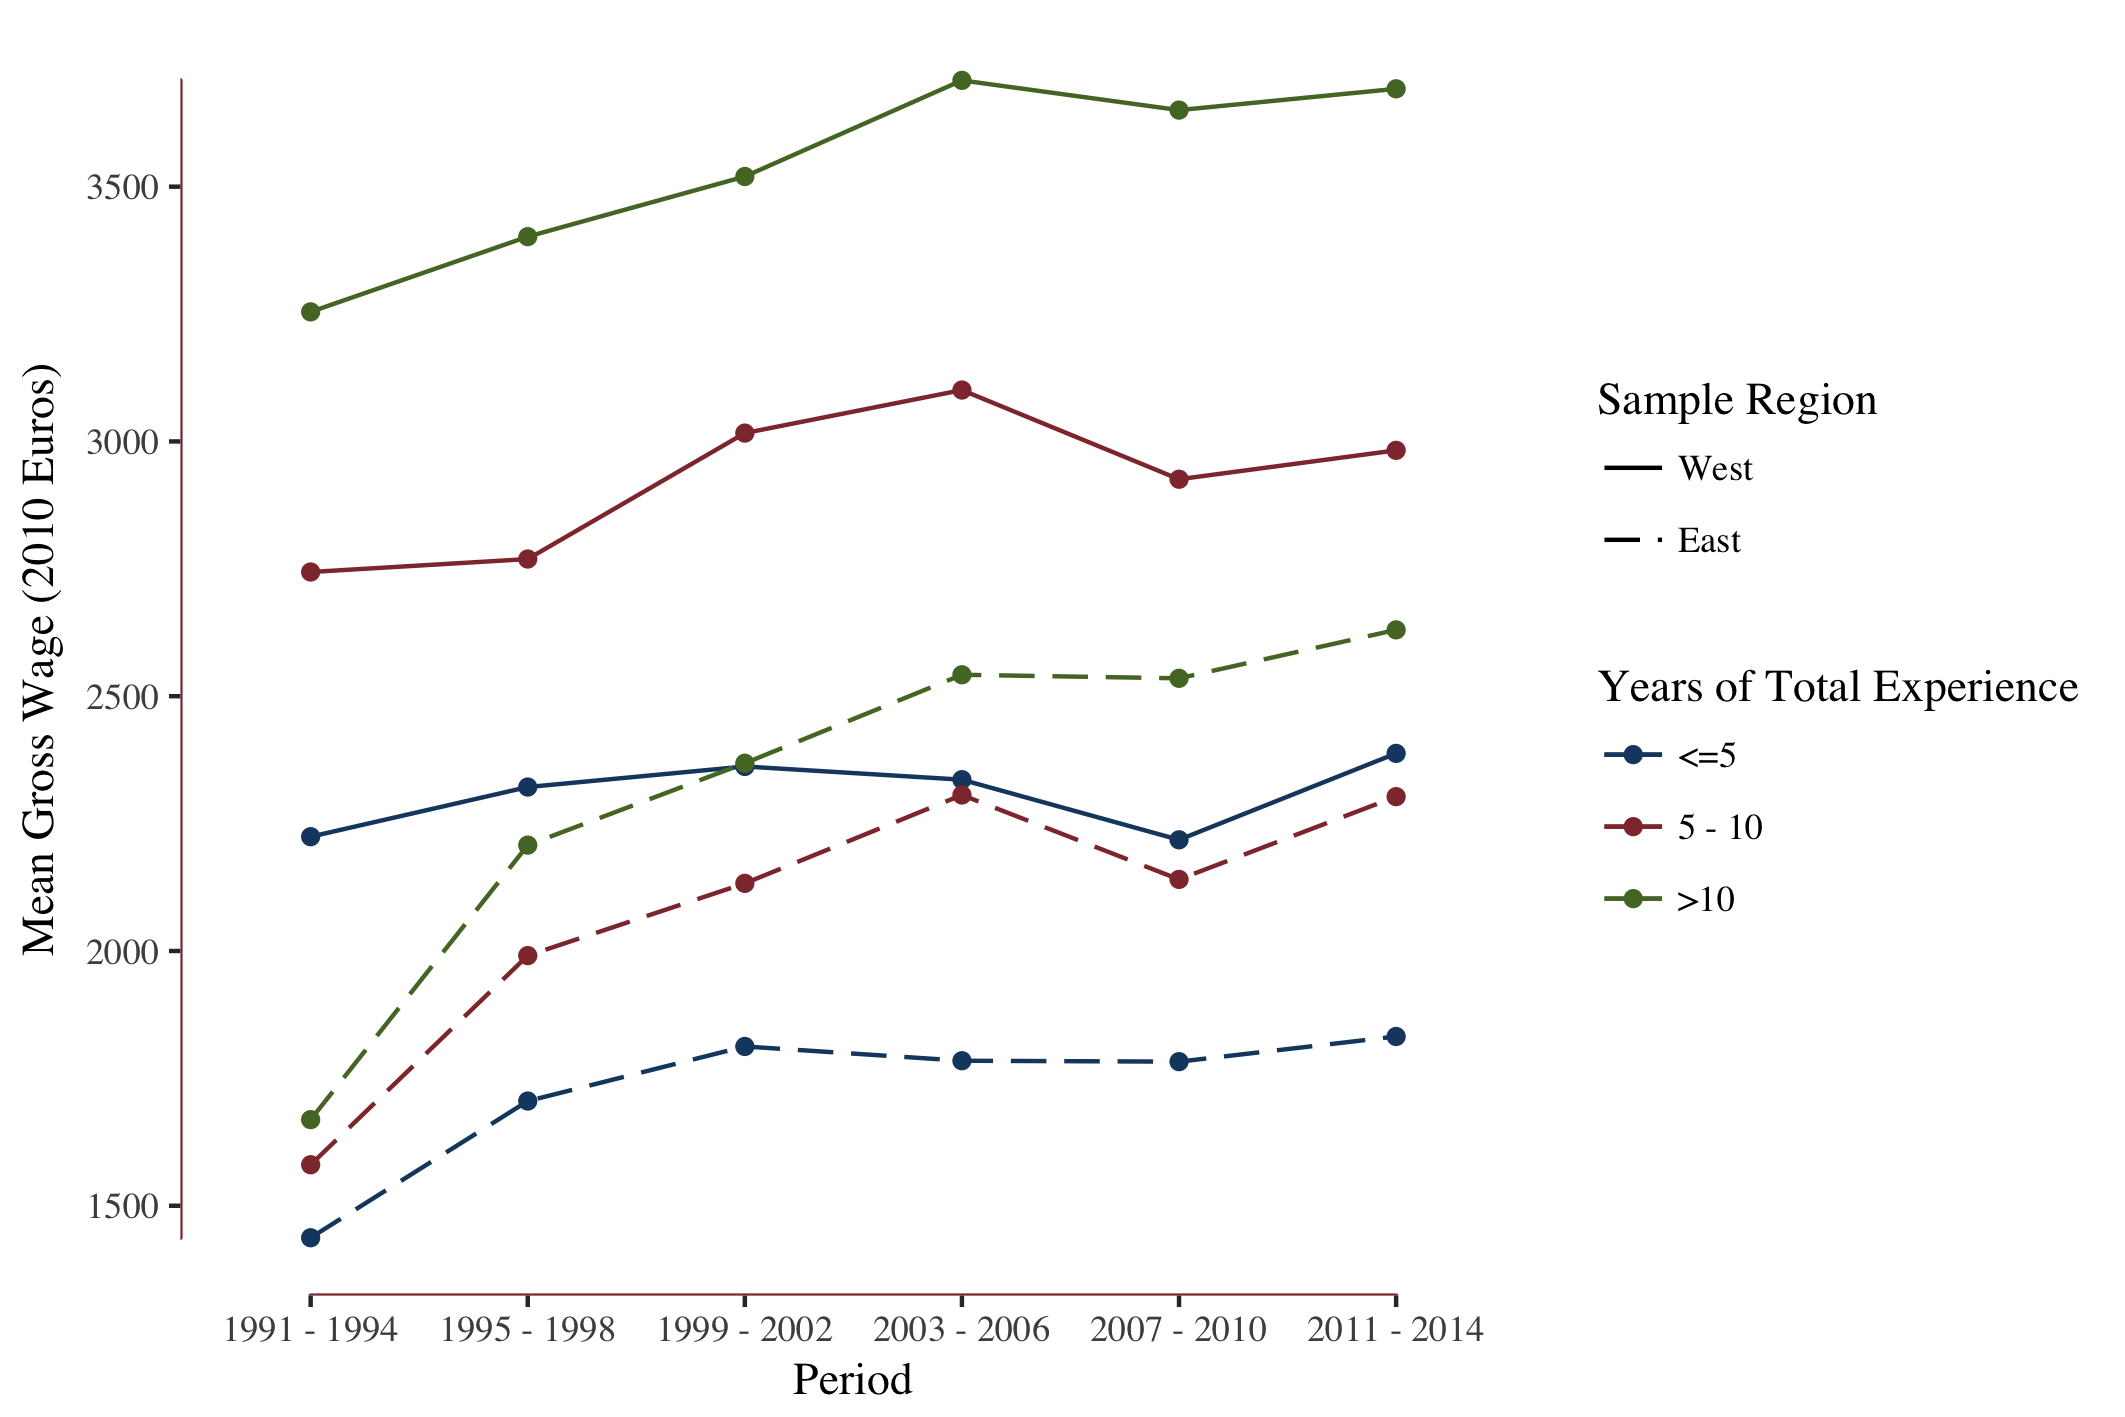
\includegraphics[width=\textwidth]{/Users/Christian/Statistik_Studium/EconProject/Code/Graphics/plotMeanWagesByTotalExp.png}
    \caption{Average Wages by Total Experience}
    \label{fig:MeanWagesByTotalExp}
\end{figure}

\begin{figure}[!h]
    \centering
    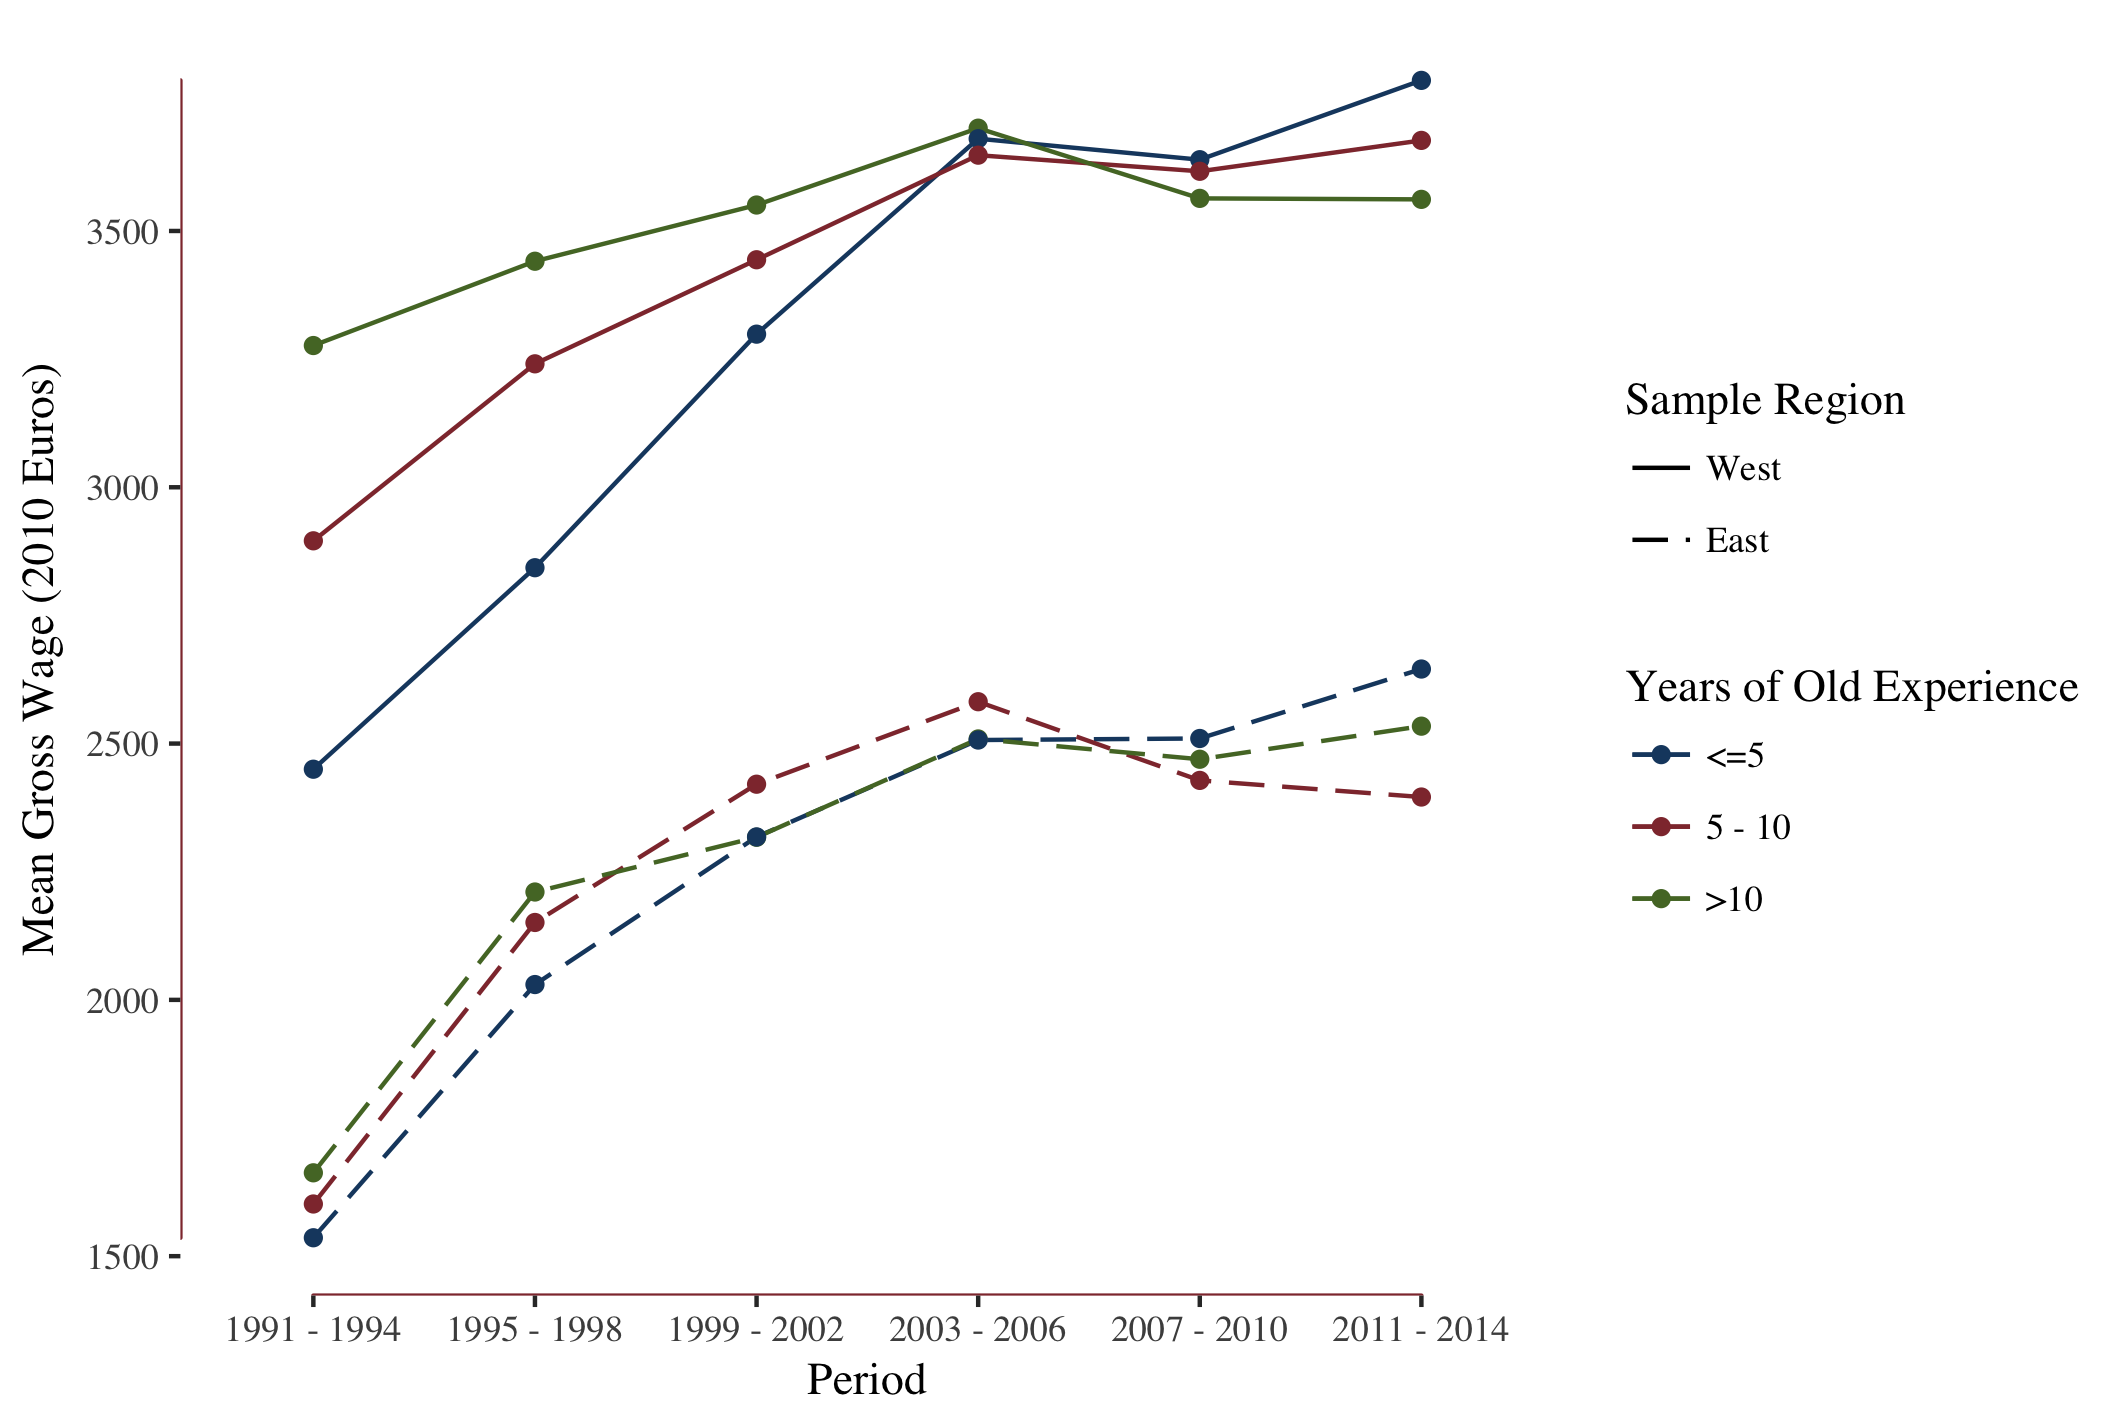
\includegraphics[width=\textwidth]{/Users/Christian/Statistik_Studium/EconProject/Code/Graphics/plotMeanWagesByOldExp.png}
    \caption{Average Wages by Old Experience}
    \label{fig:MeanWagesByOldExp}
\end{figure}

\begin{figure}[!h]
    \centering
    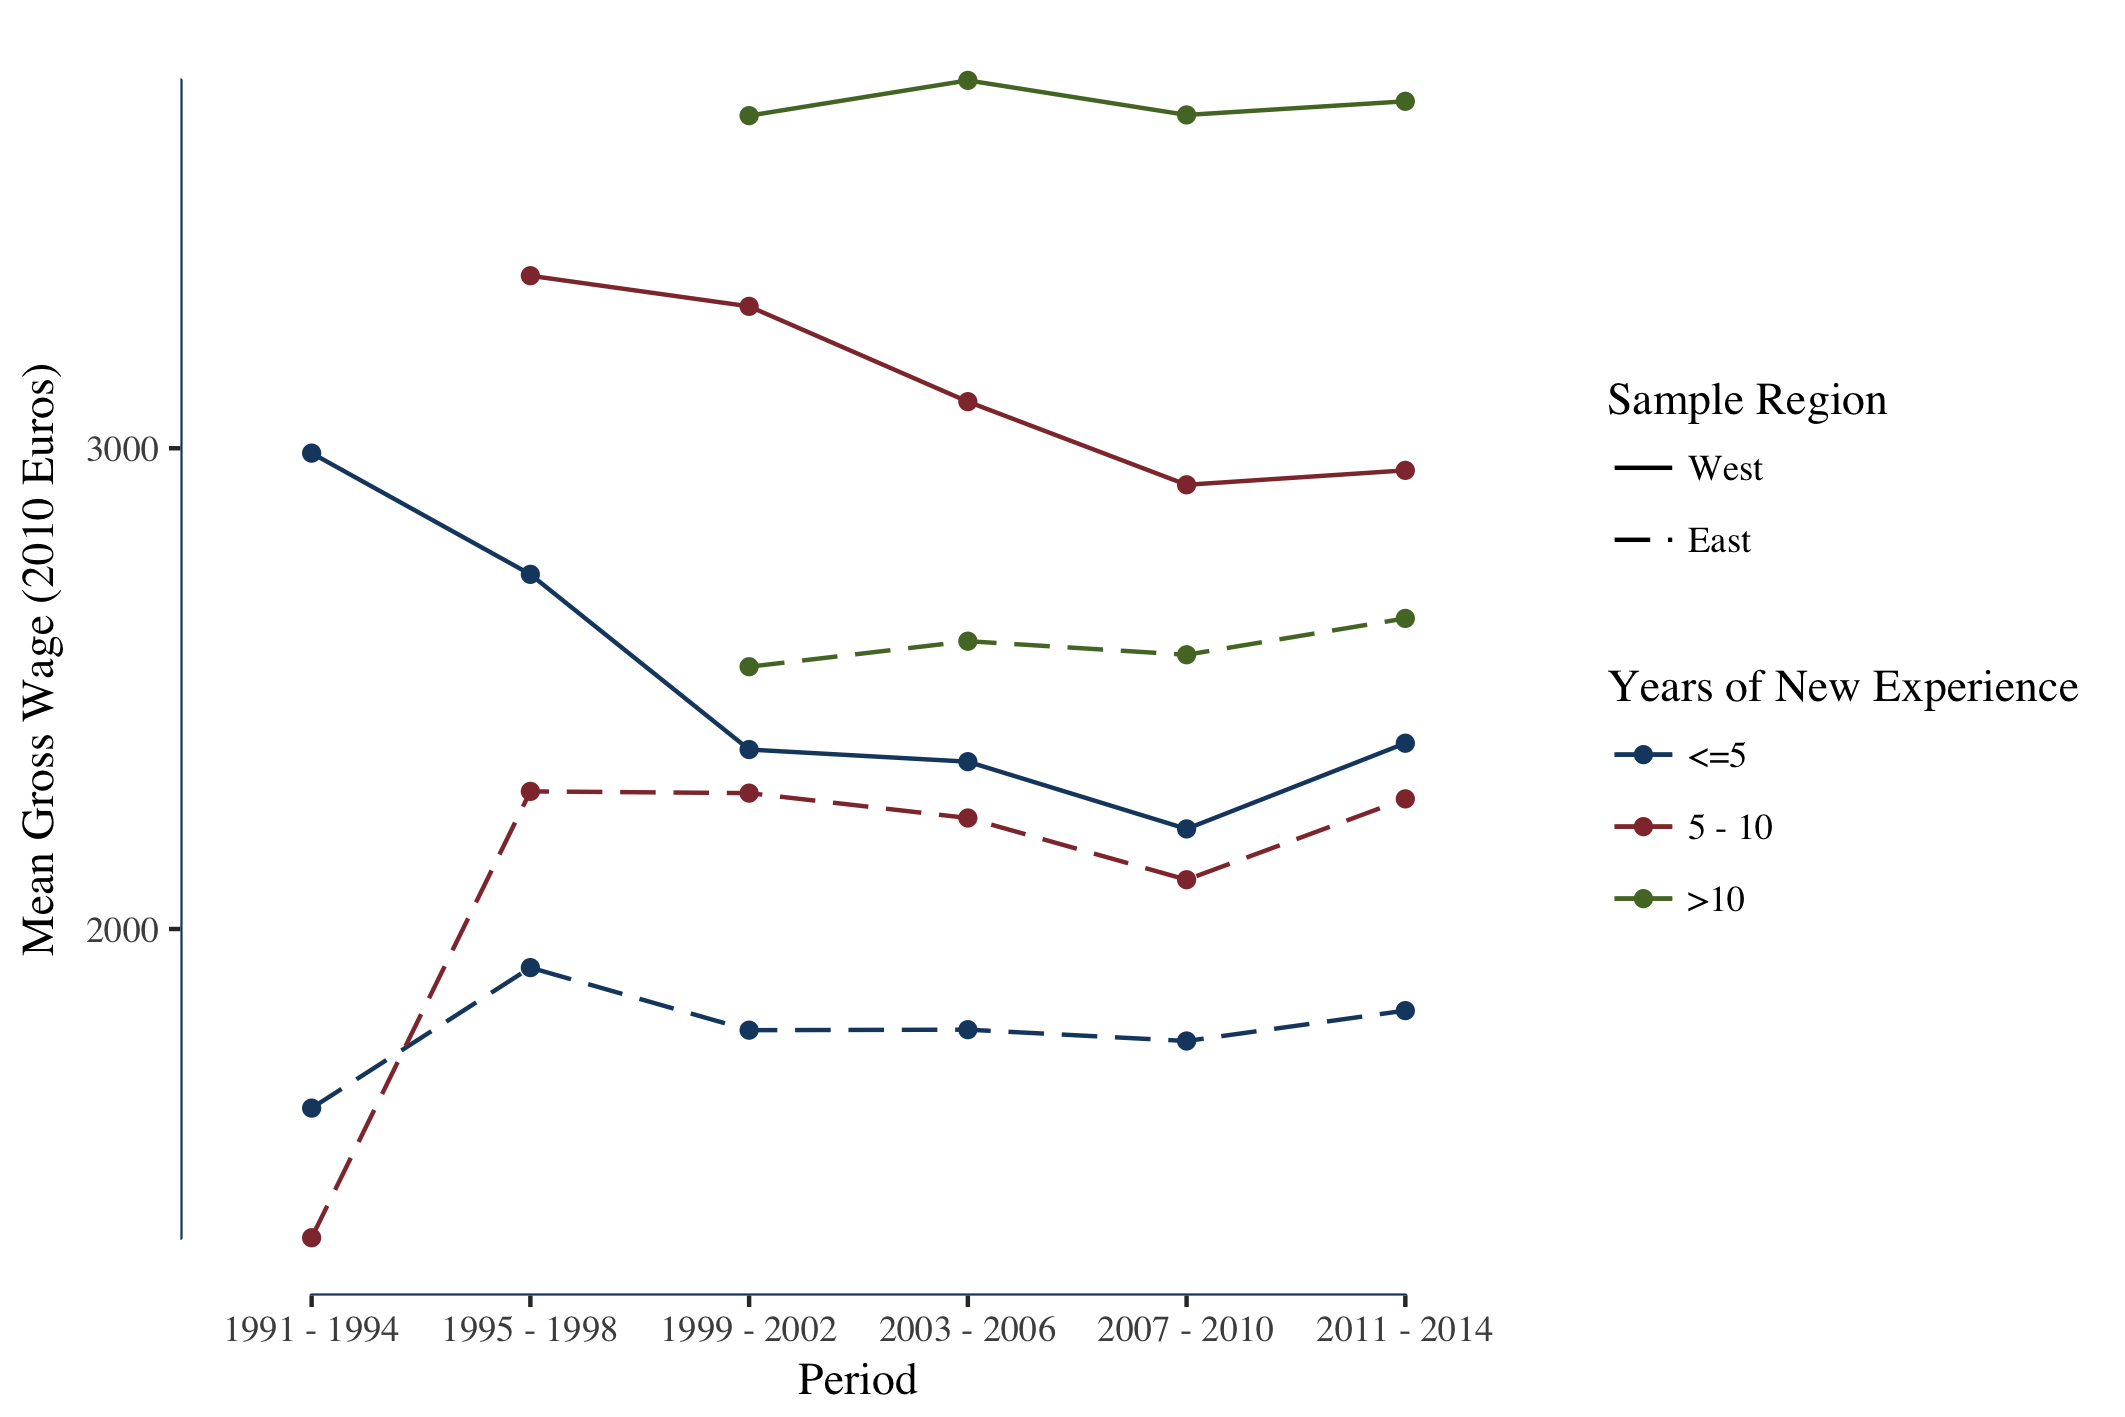
\includegraphics[width=\textwidth]{/Users/Christian/Statistik_Studium/EconProject/Code/Graphics/plotMeanWagesByNewExp.png}
    \caption{Average Wages by New Experience}
    \label{fig:MeanWagesByNewExp}
\end{figure}

\begin{figure}[!h]
    \centering
    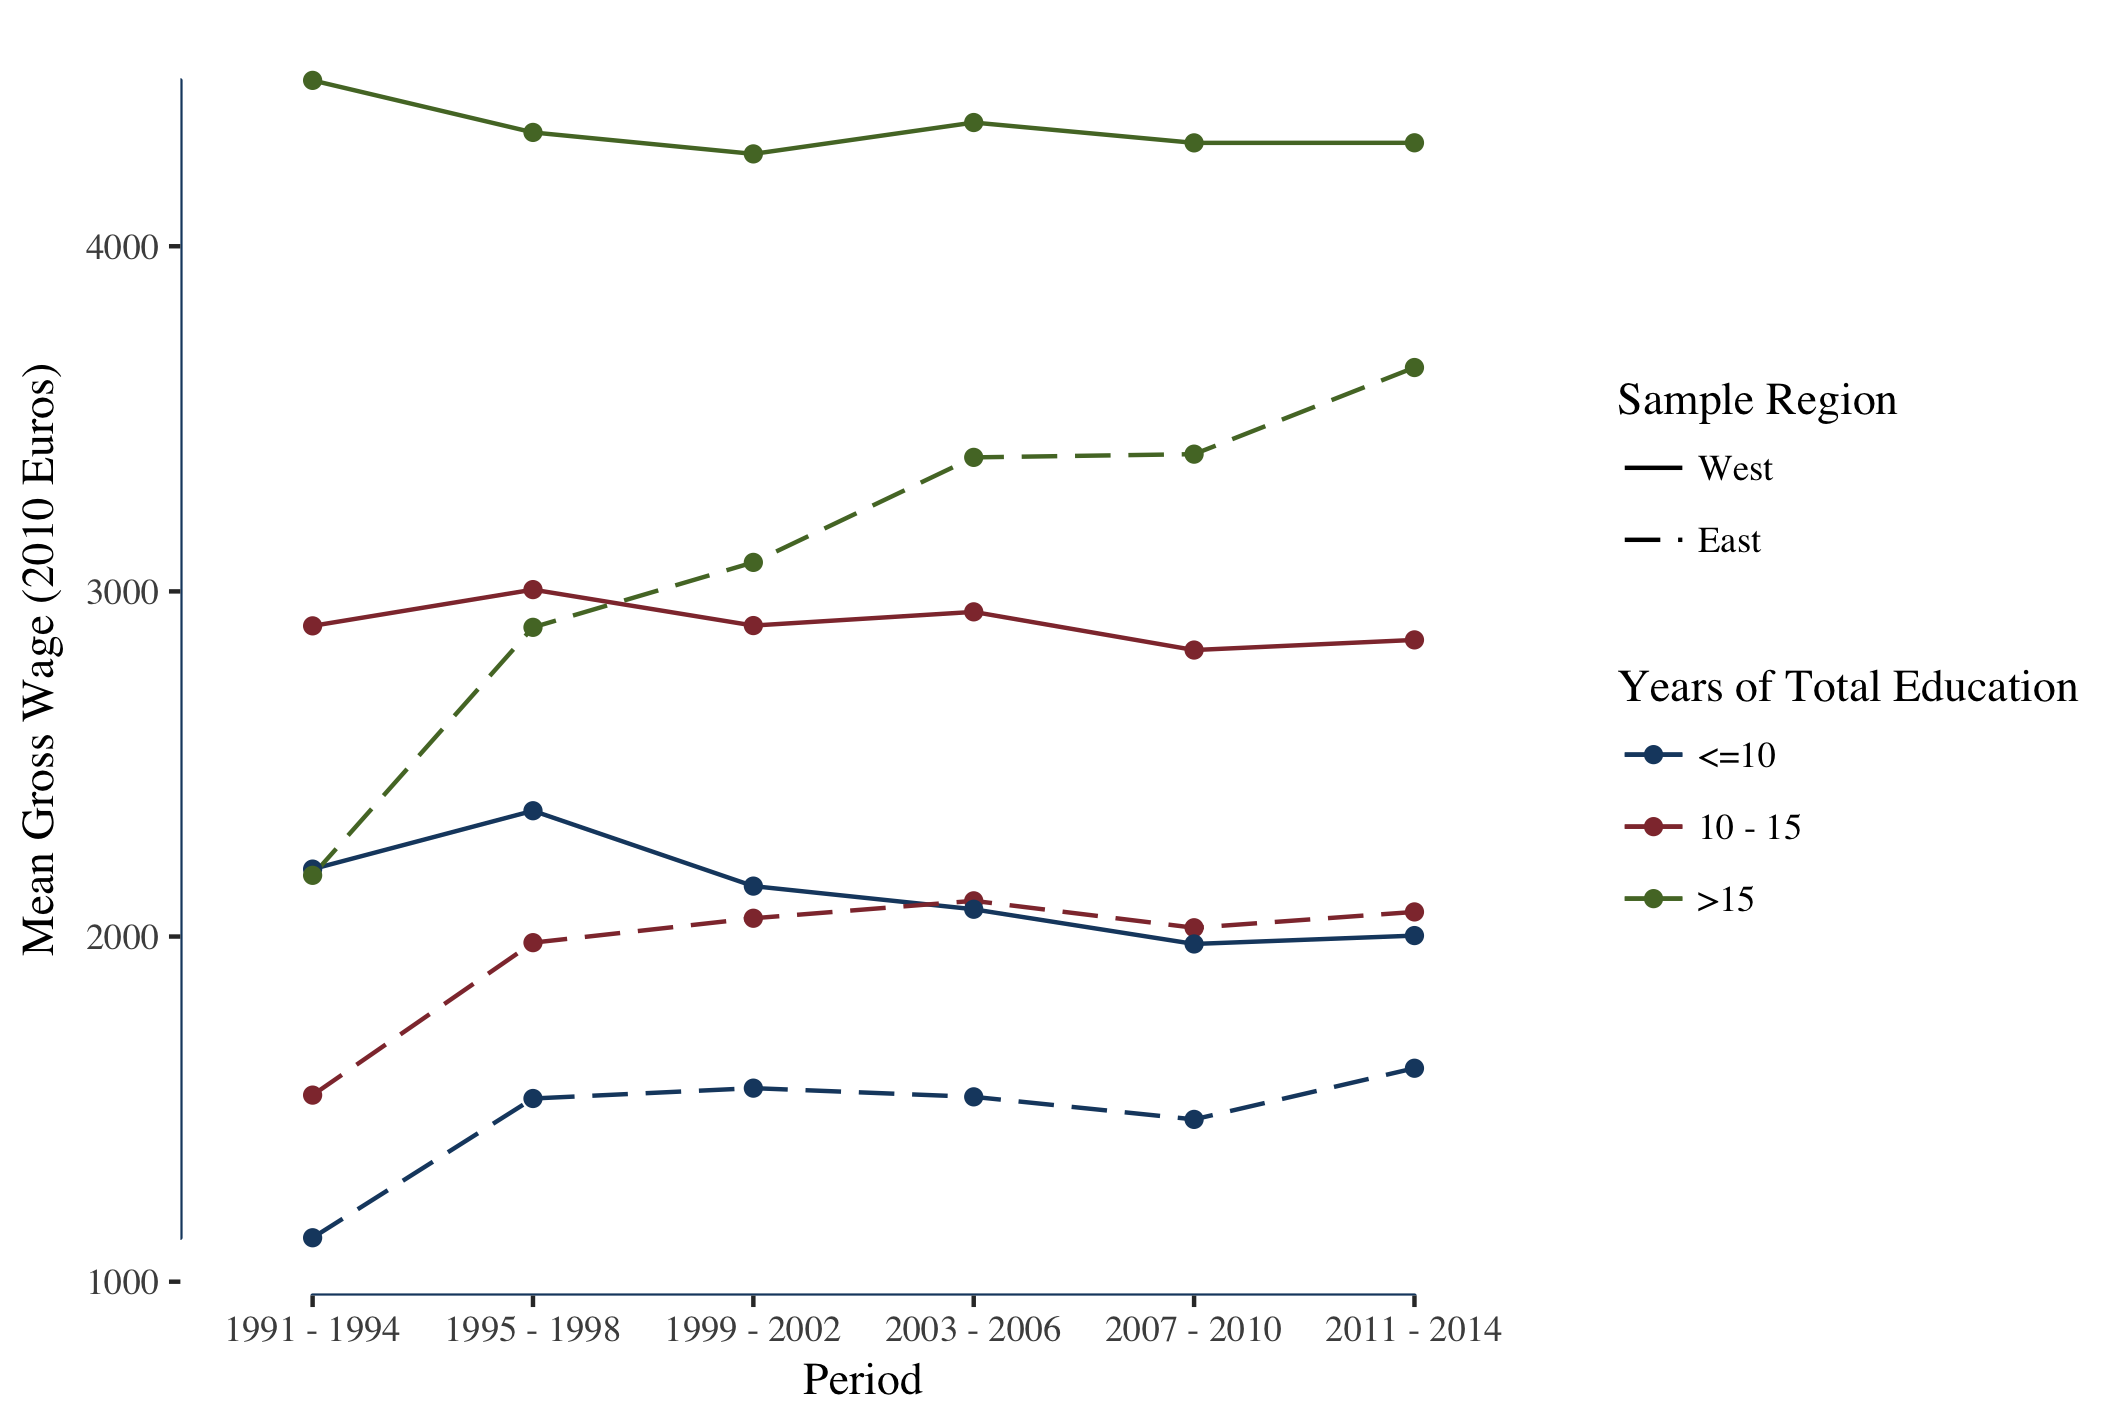
\includegraphics[width=\textwidth]{/Users/Christian/Statistik_Studium/EconProject/Code/Graphics/plotMeanWagesByTotalEdu.png}
    \caption{Average Wages by Total Education}
    \label{fig:MeanWagesByTotalEdu}
\end{figure}

\begin{figure}[!h]
    \centering
    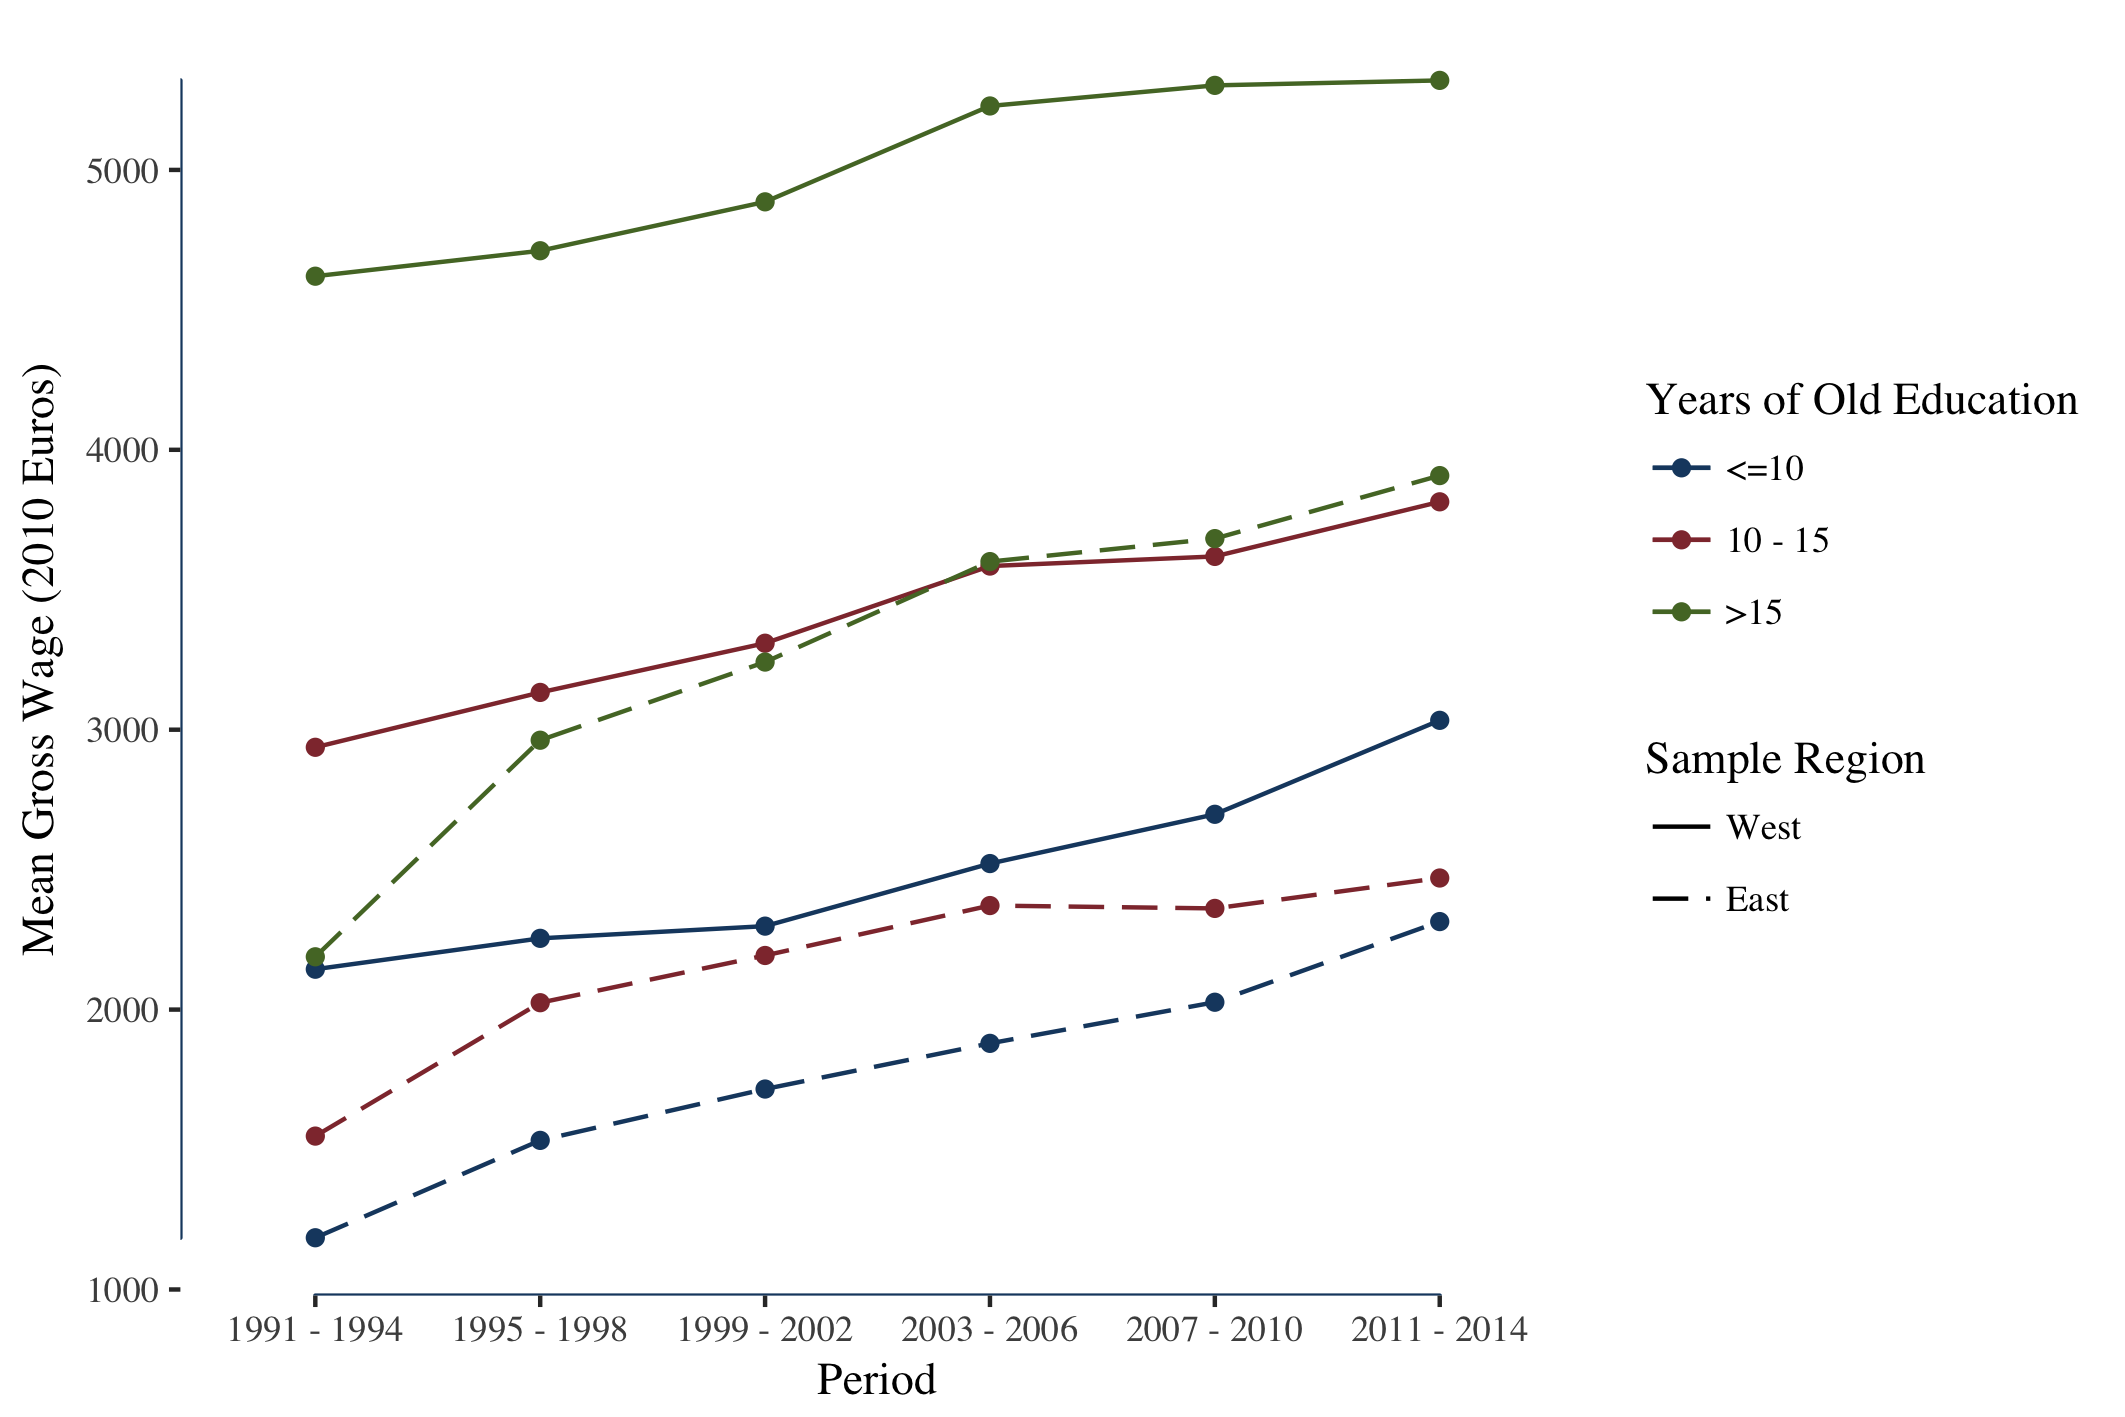
\includegraphics[width=\textwidth]{/Users/Christian/Statistik_Studium/EconProject/Code/Graphics/plotMeanWagesByOldEdu.png}
    \caption{Average Wages by Old Education}
    \label{fig:MeanWagesByOldEdu}
\end{figure}

\begin{figure}[!h]
    \centering
    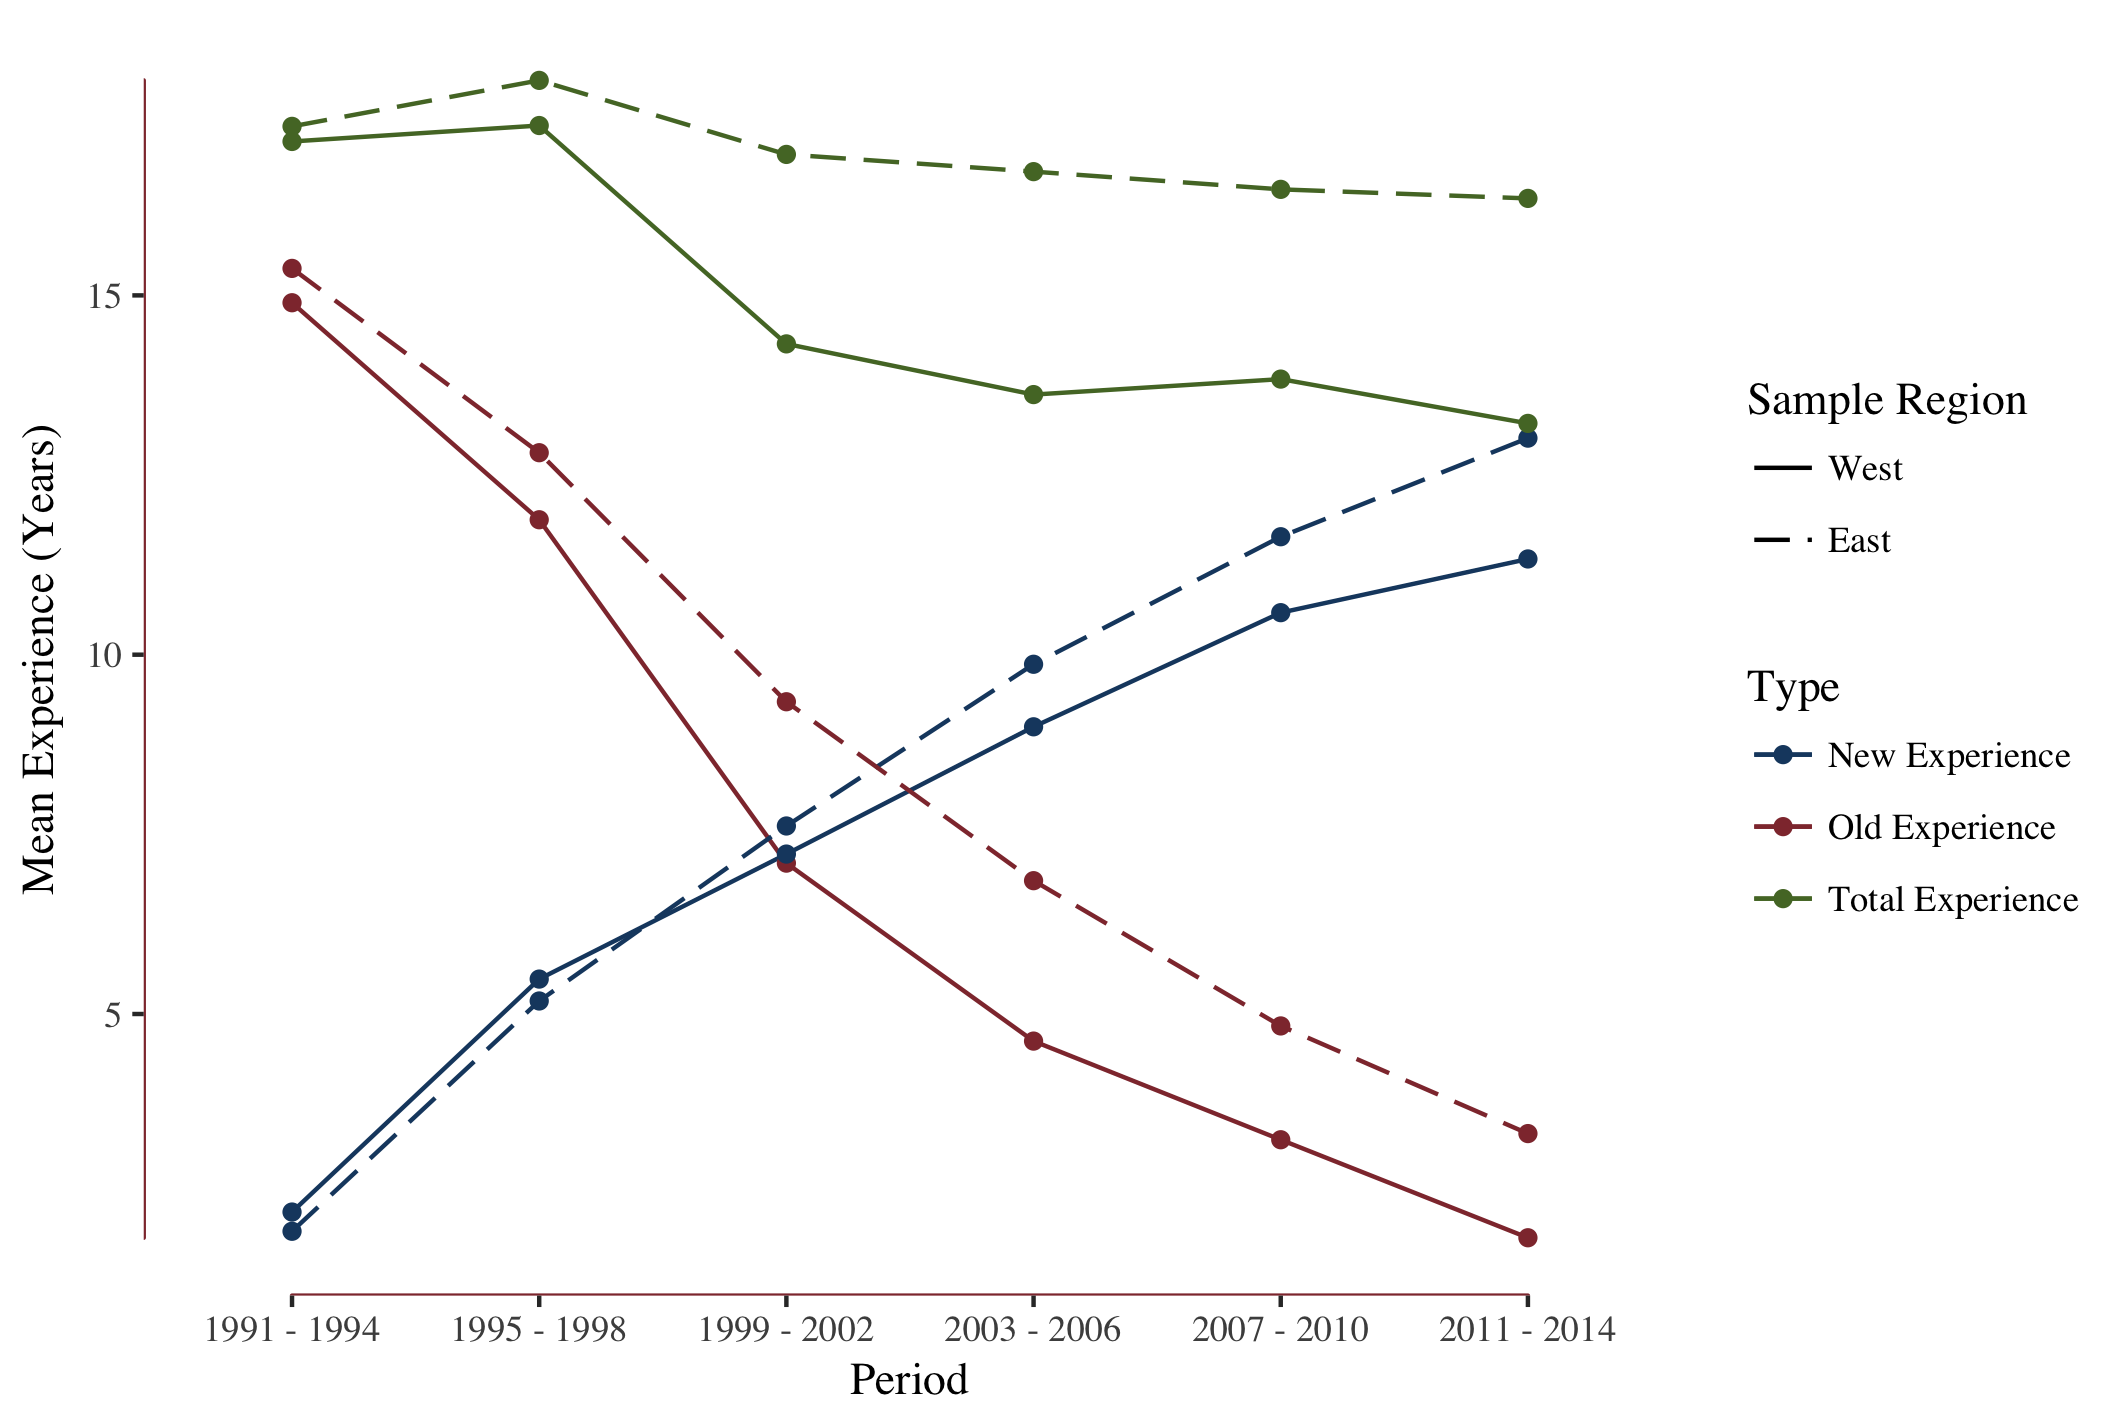
\includegraphics[width=\textwidth]{/Users/Christian/Statistik_Studium/EconProject/Code/Graphics/plotMeanExp.png}
    \caption{Average Years of Experience}
    \label{fig:MeanExp}
\end{figure}

\begin{figure}[!h]
    \centering
    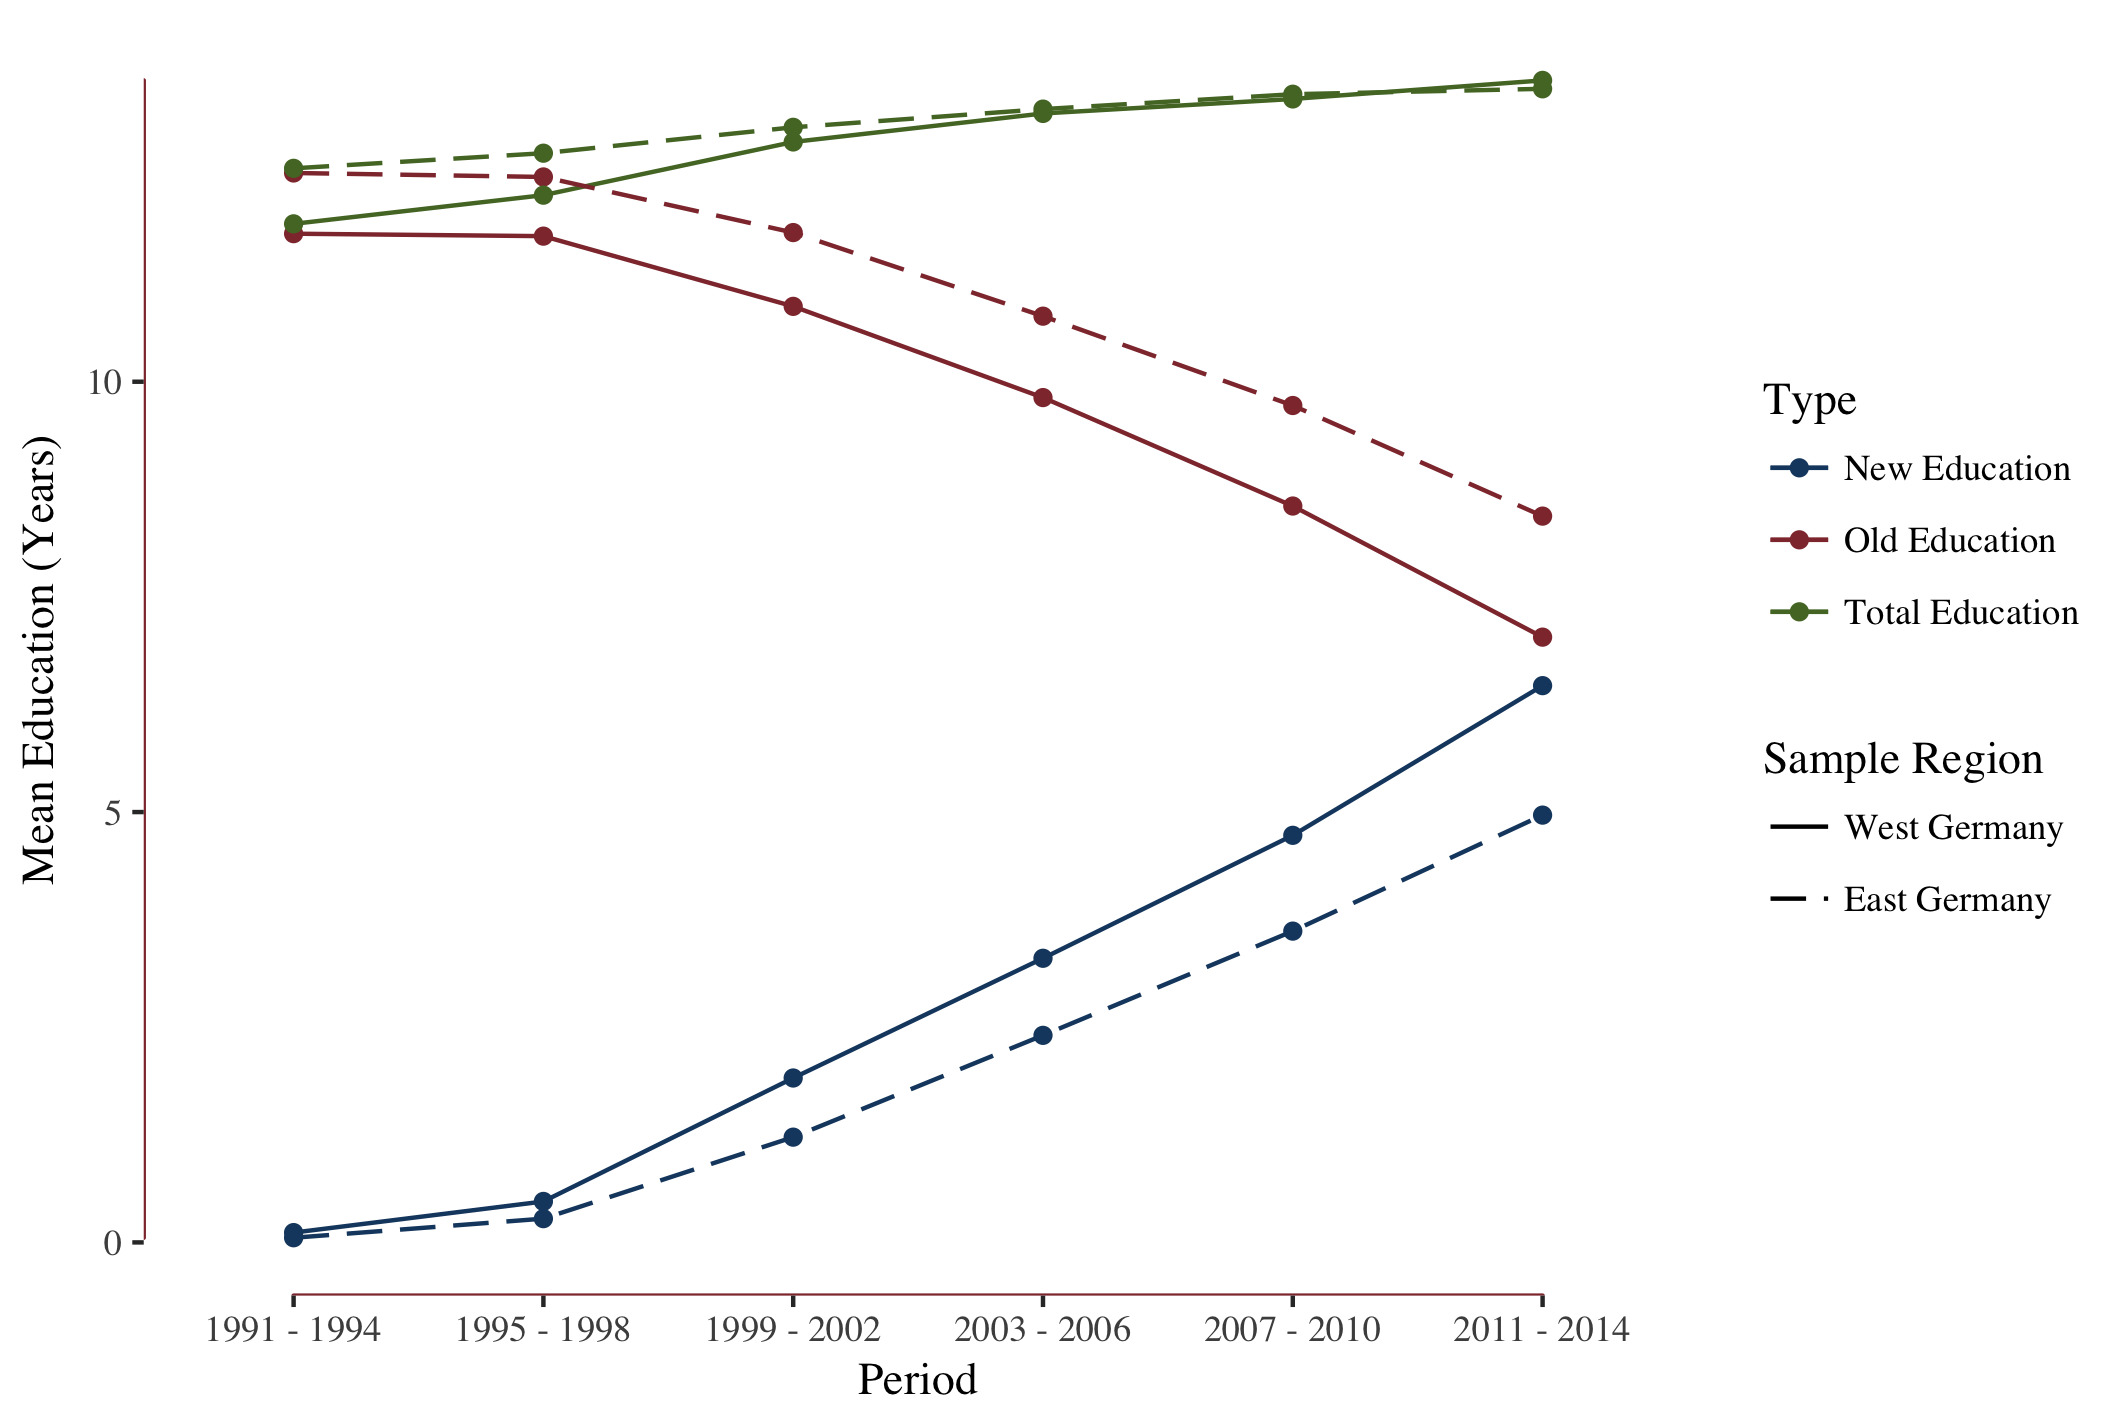
\includegraphics[width=\textwidth]{/Users/Christian/Statistik_Studium/EconProject/Code/Graphics/plotMeanEdu.png}
    \caption{Average Years of Education}
    \label{fig:MeanEdu}
\end{figure}

\begin{figure}[!h]
    \centering
    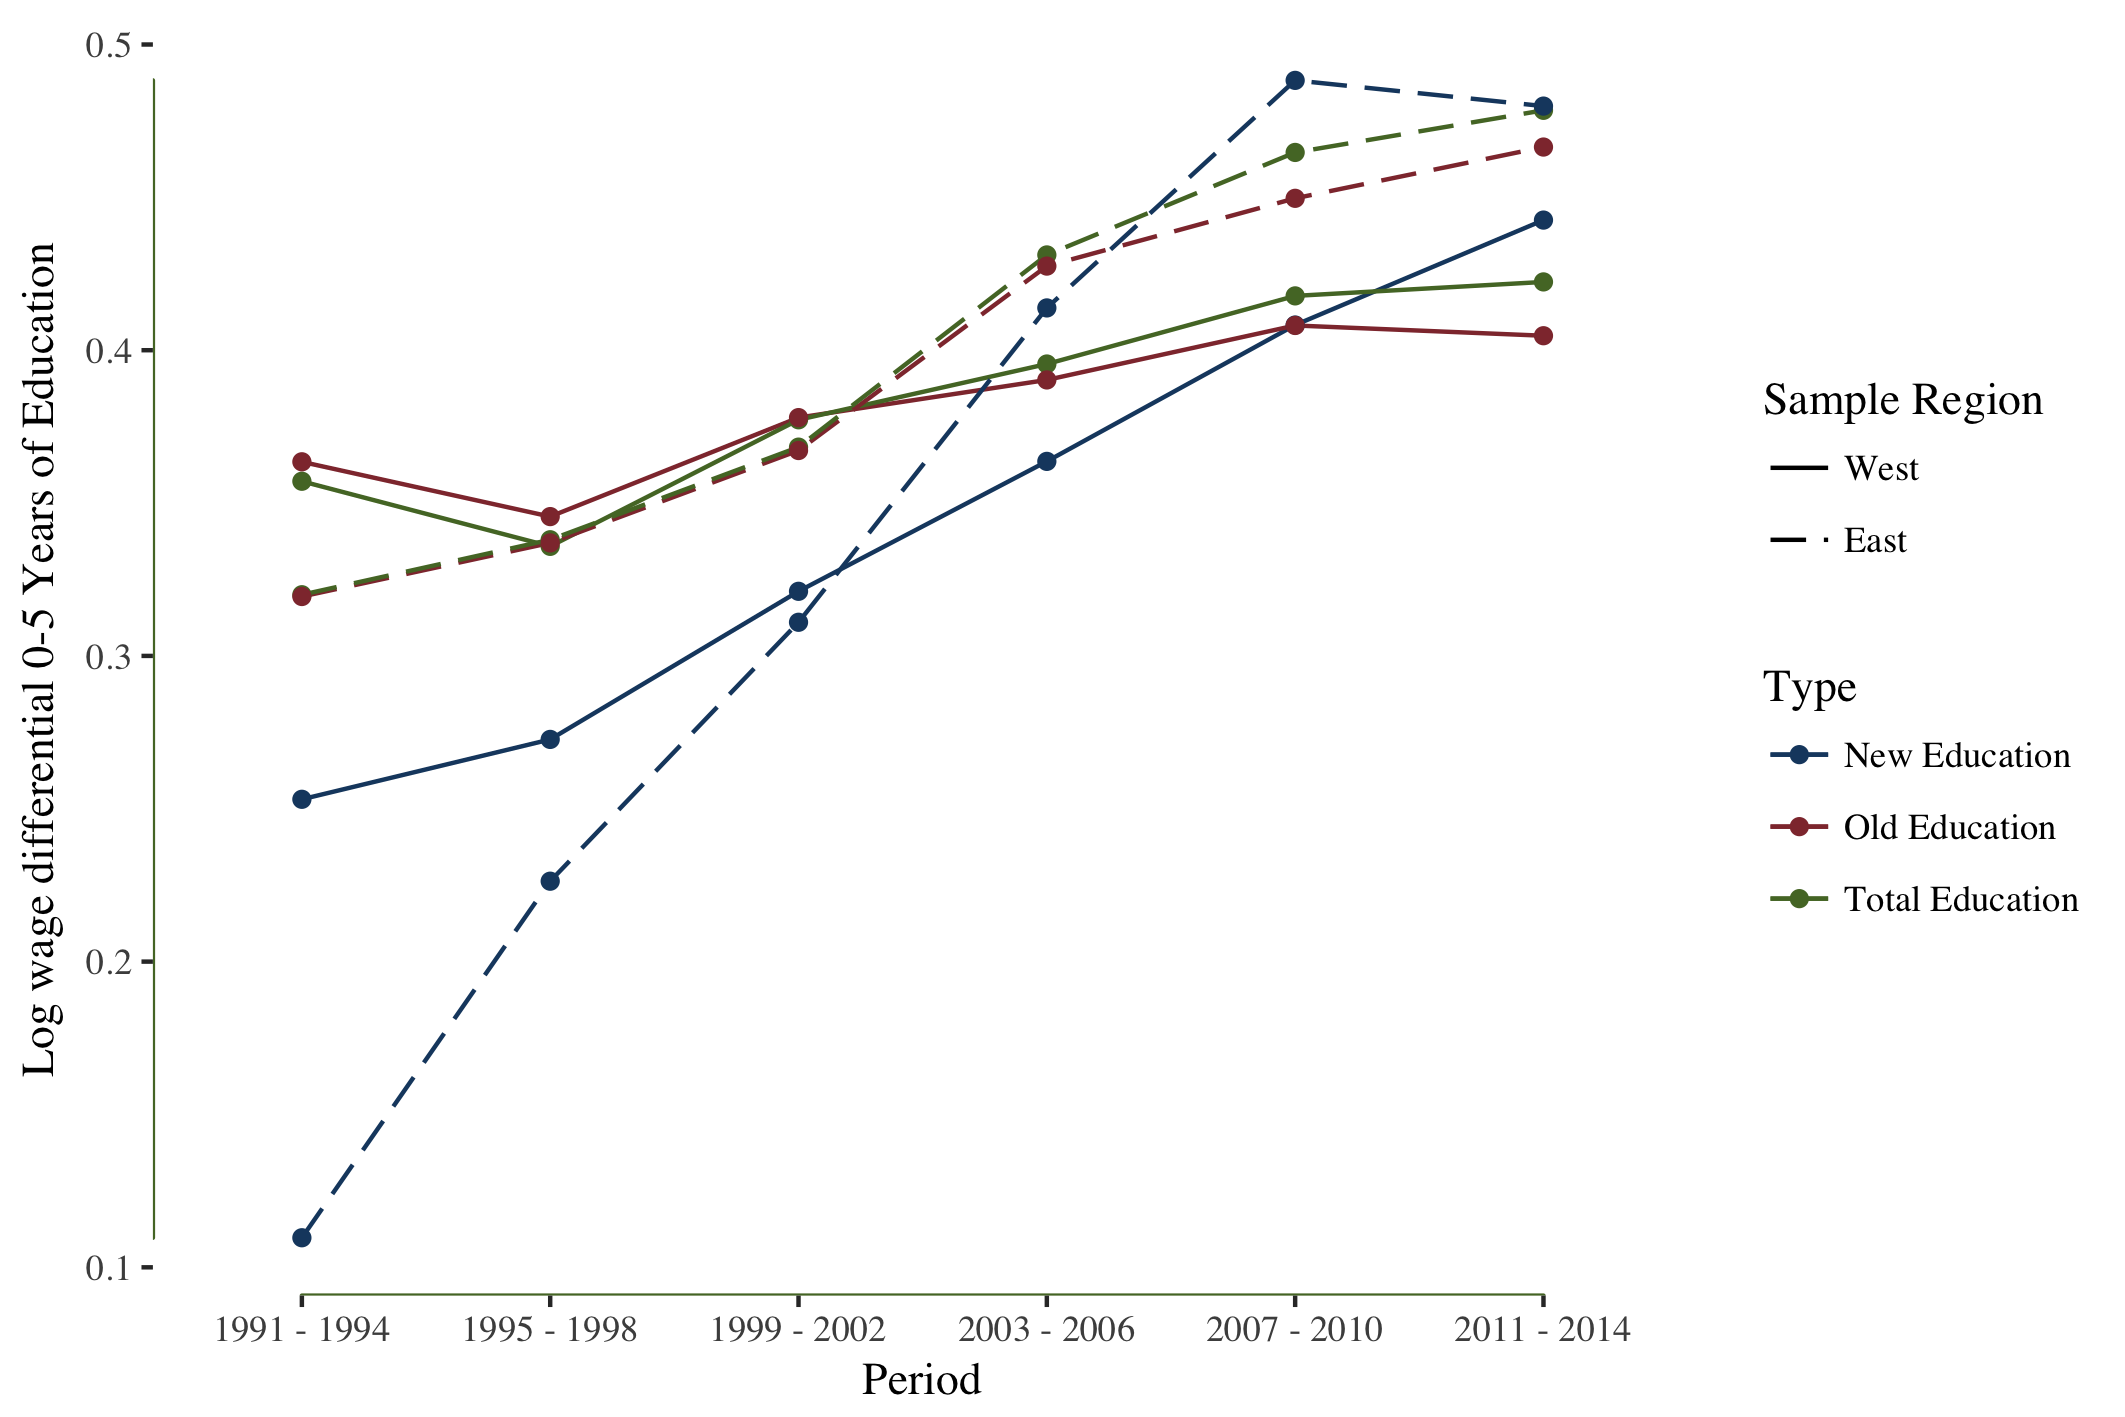
\includegraphics[width=\textwidth]{/Users/Christian/Statistik_Studium/EconProject/Code/Graphics/plotDiffComparisonEdu.png}
    \caption{Returns to  Education}
    \label{fig:DiffComparisonEdu}
\end{figure}

\begin{figure}[!h]
    \centering
    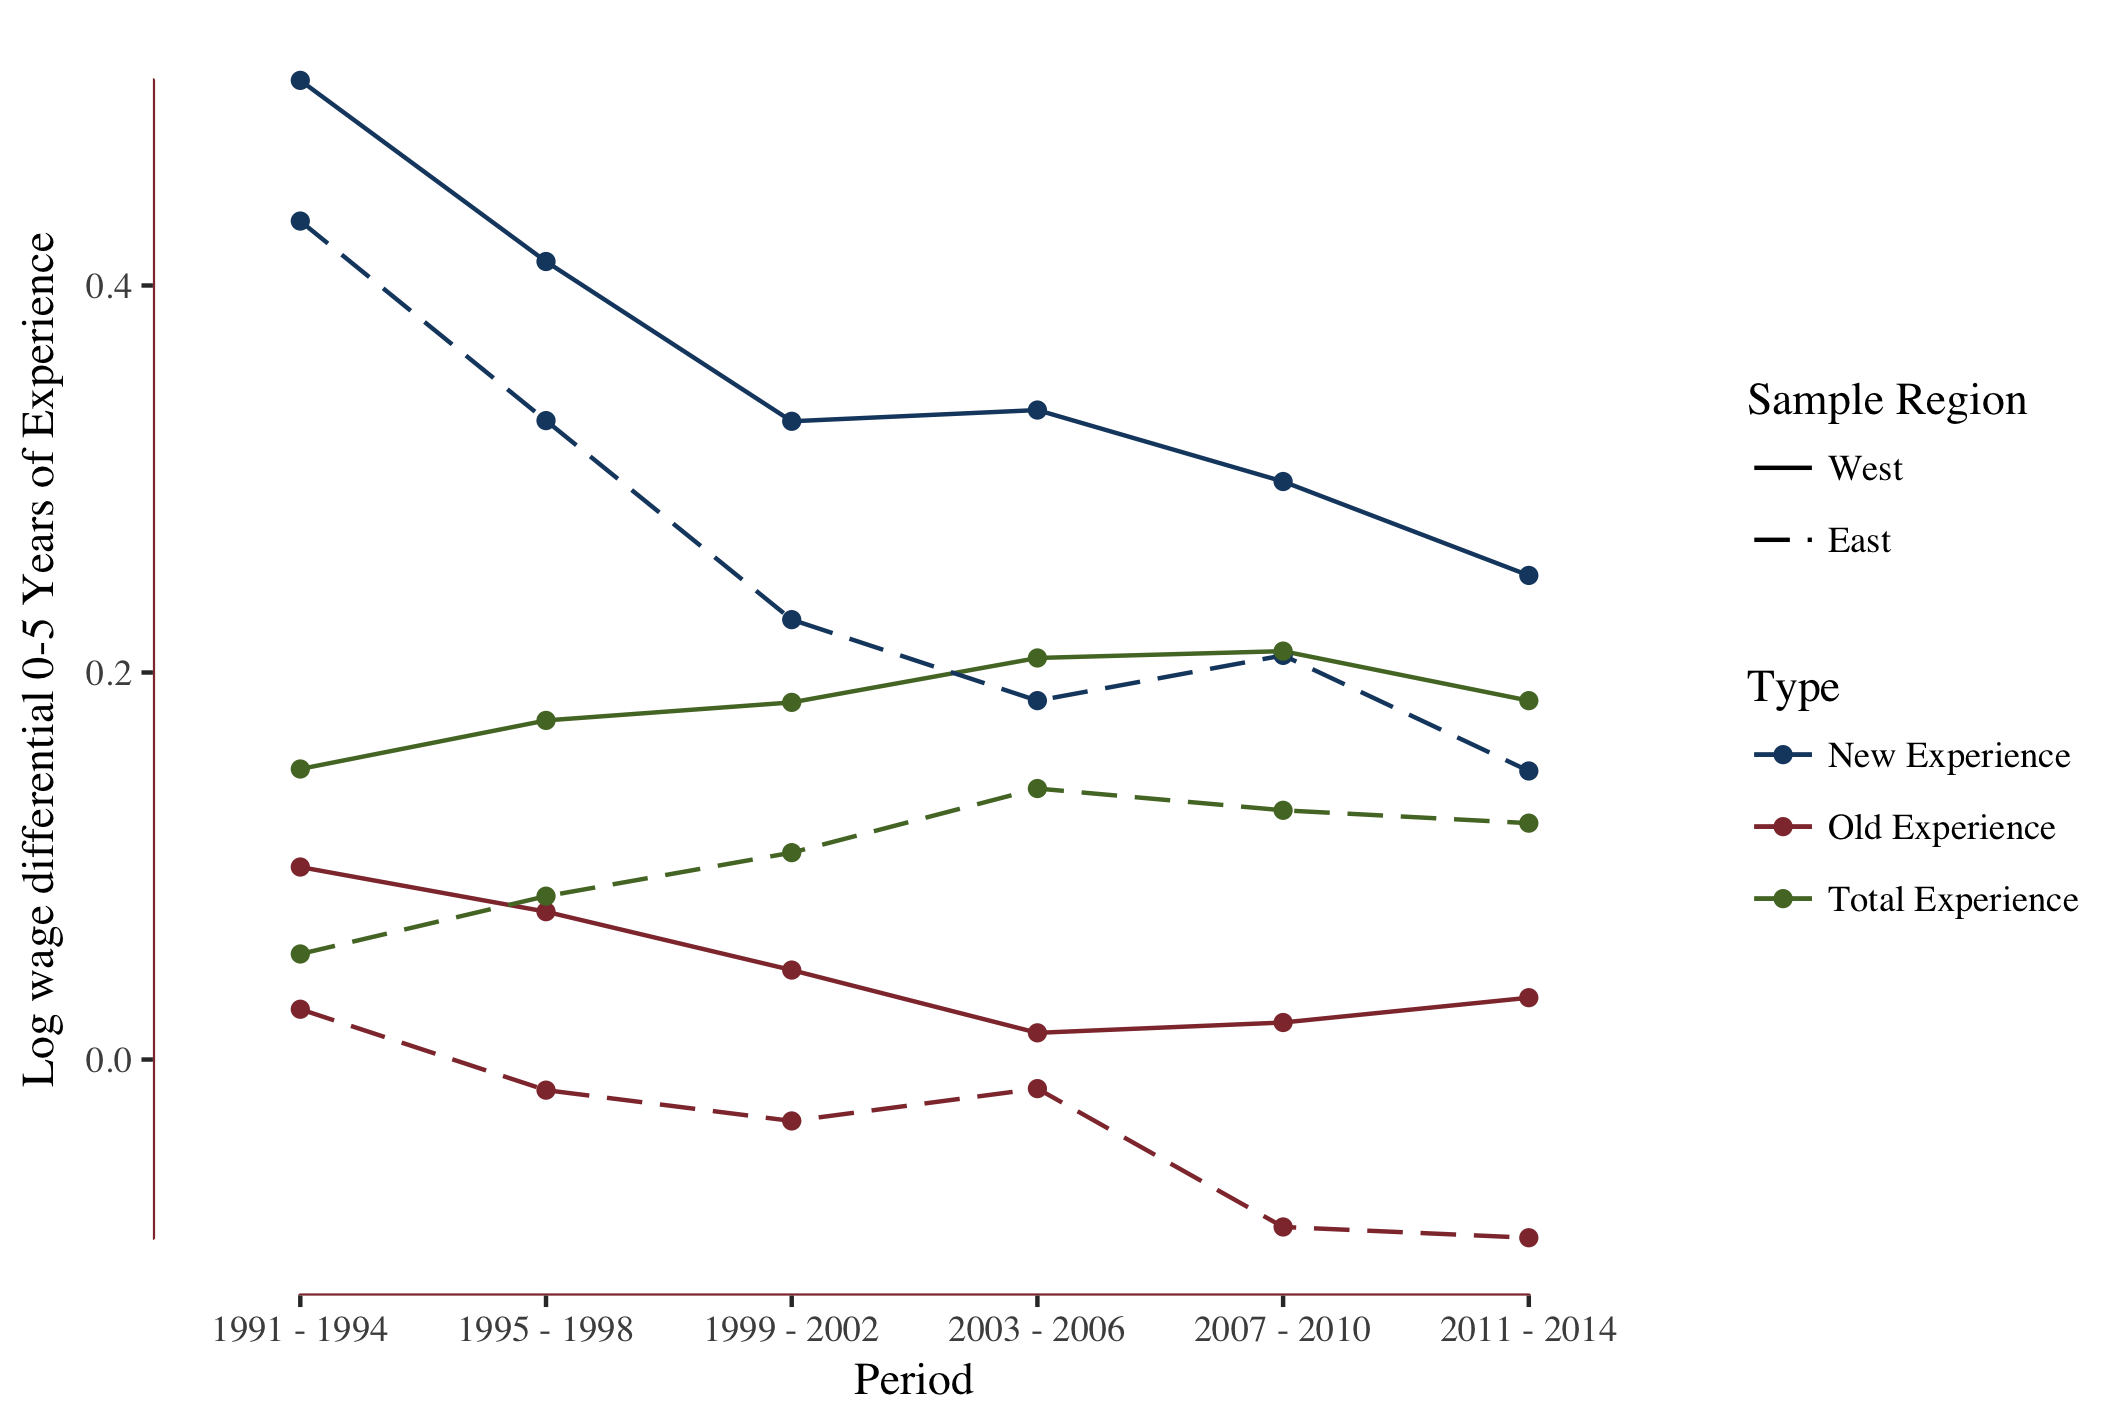
\includegraphics[width=\textwidth]{/Users/Christian/Statistik_Studium/EconProject/Code/Graphics/plotDiffComparisonExp.png}
    \caption{Returns to Experience}
    \label{fig:DiffComparisonExp}
\end{figure}


\begin{figure}[!h]
    \centering
    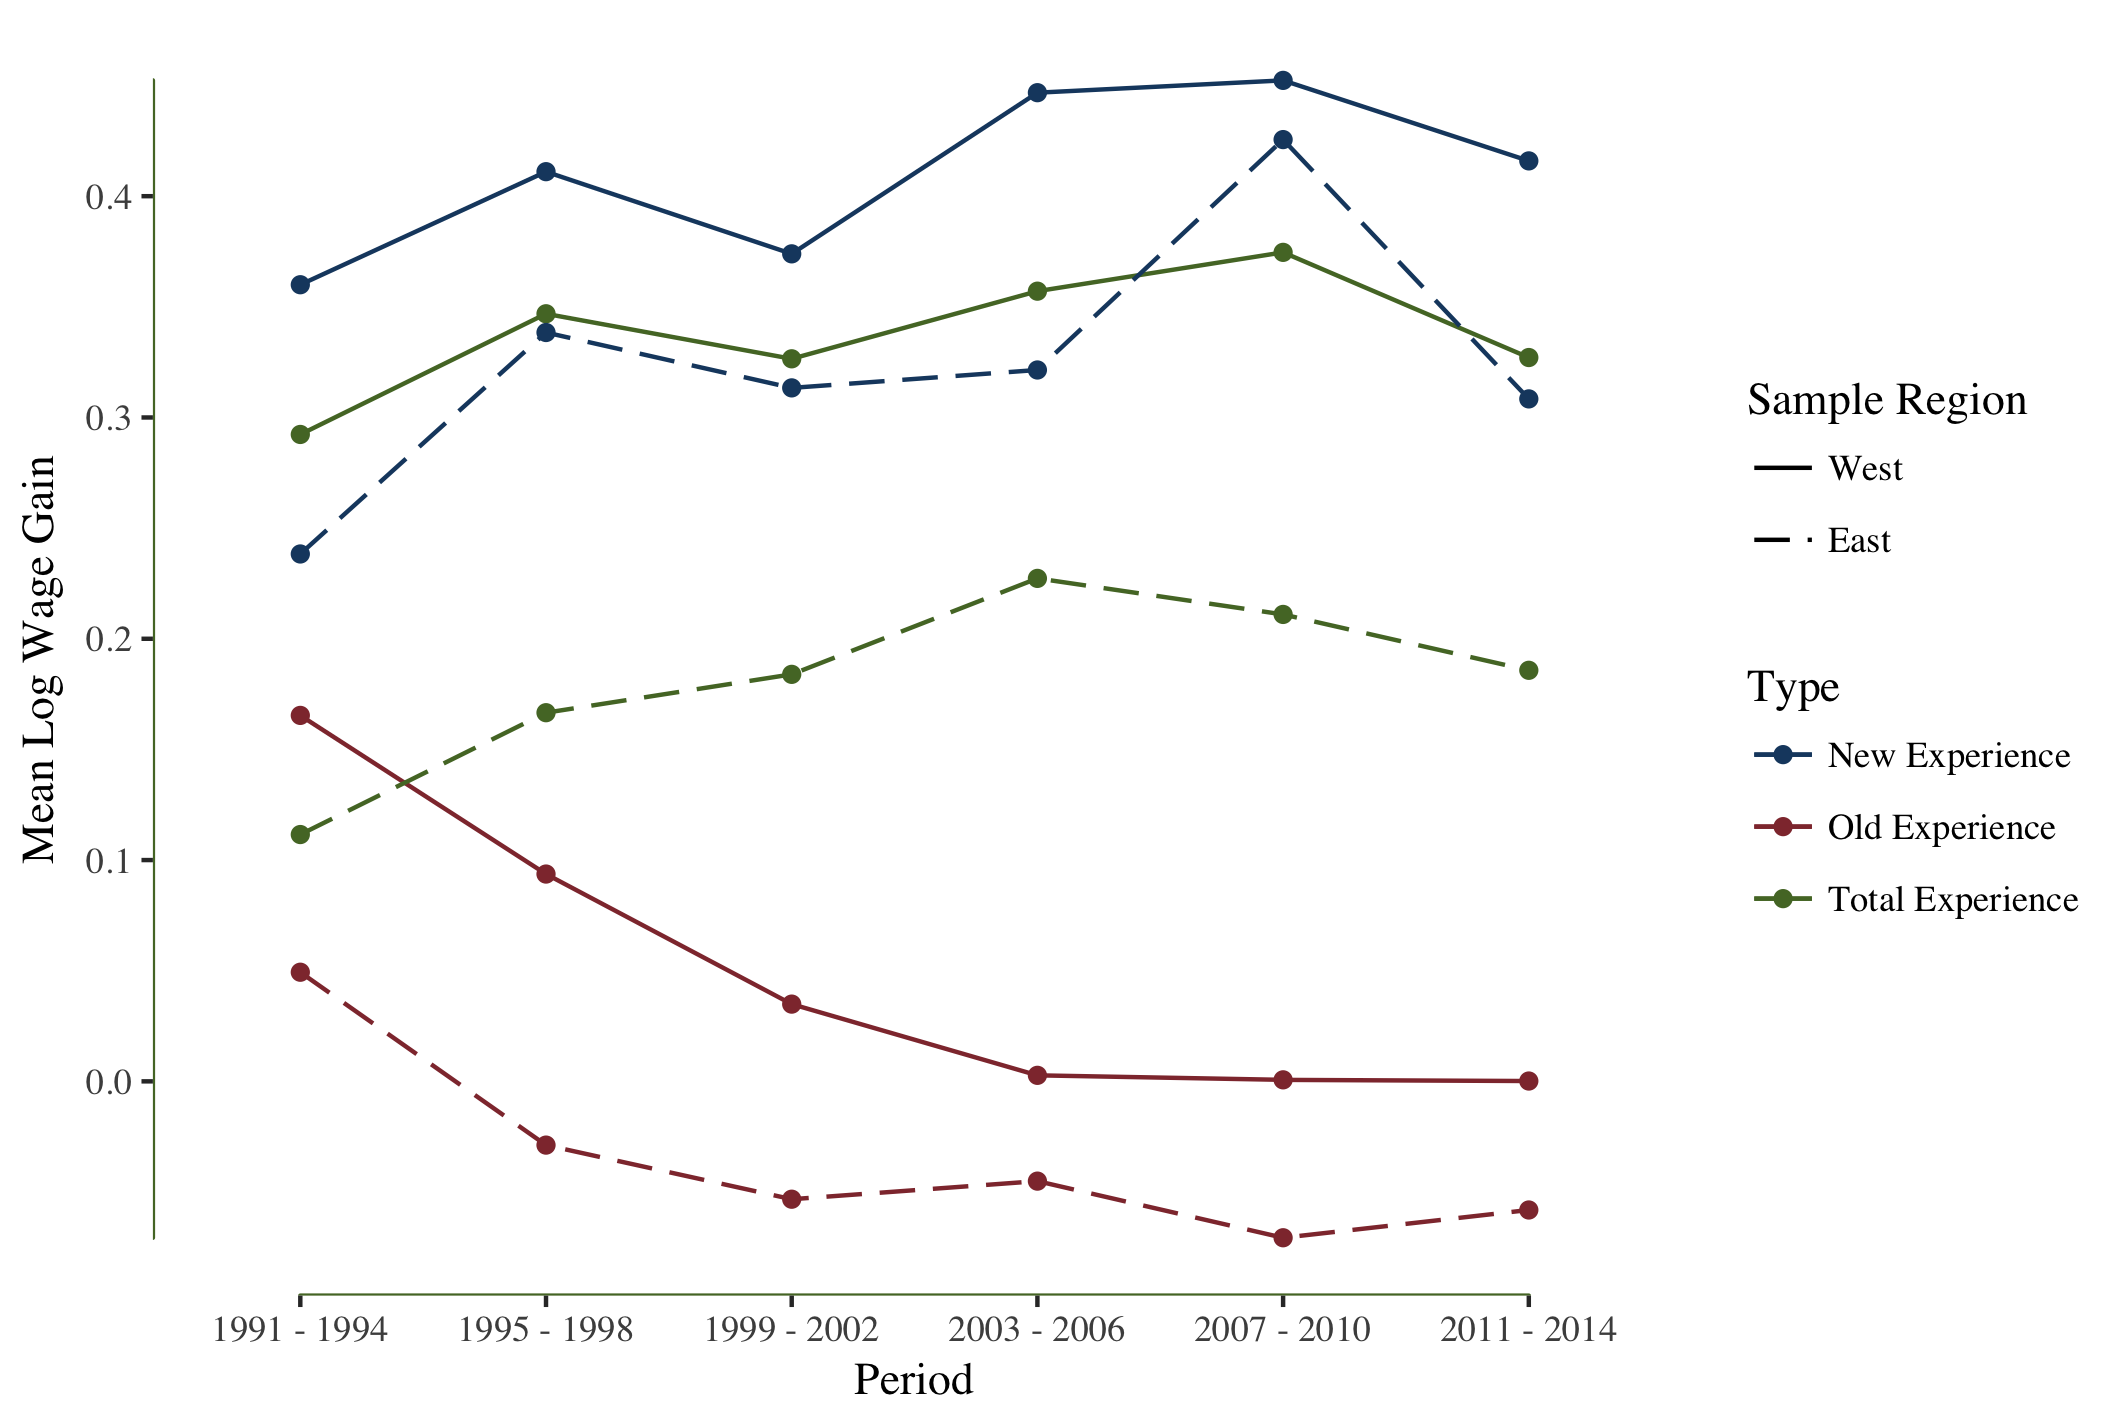
\includegraphics[width=\textwidth]{/Users/Christian/Statistik_Studium/EconProject/Code/Graphics/plotHumanCapitalExp.png}
    \caption{Average Human Capital in Experience}
    \label{fig:HumanCapitalExp}
\end{figure}

\begin{figure}[!h]
    \centering
    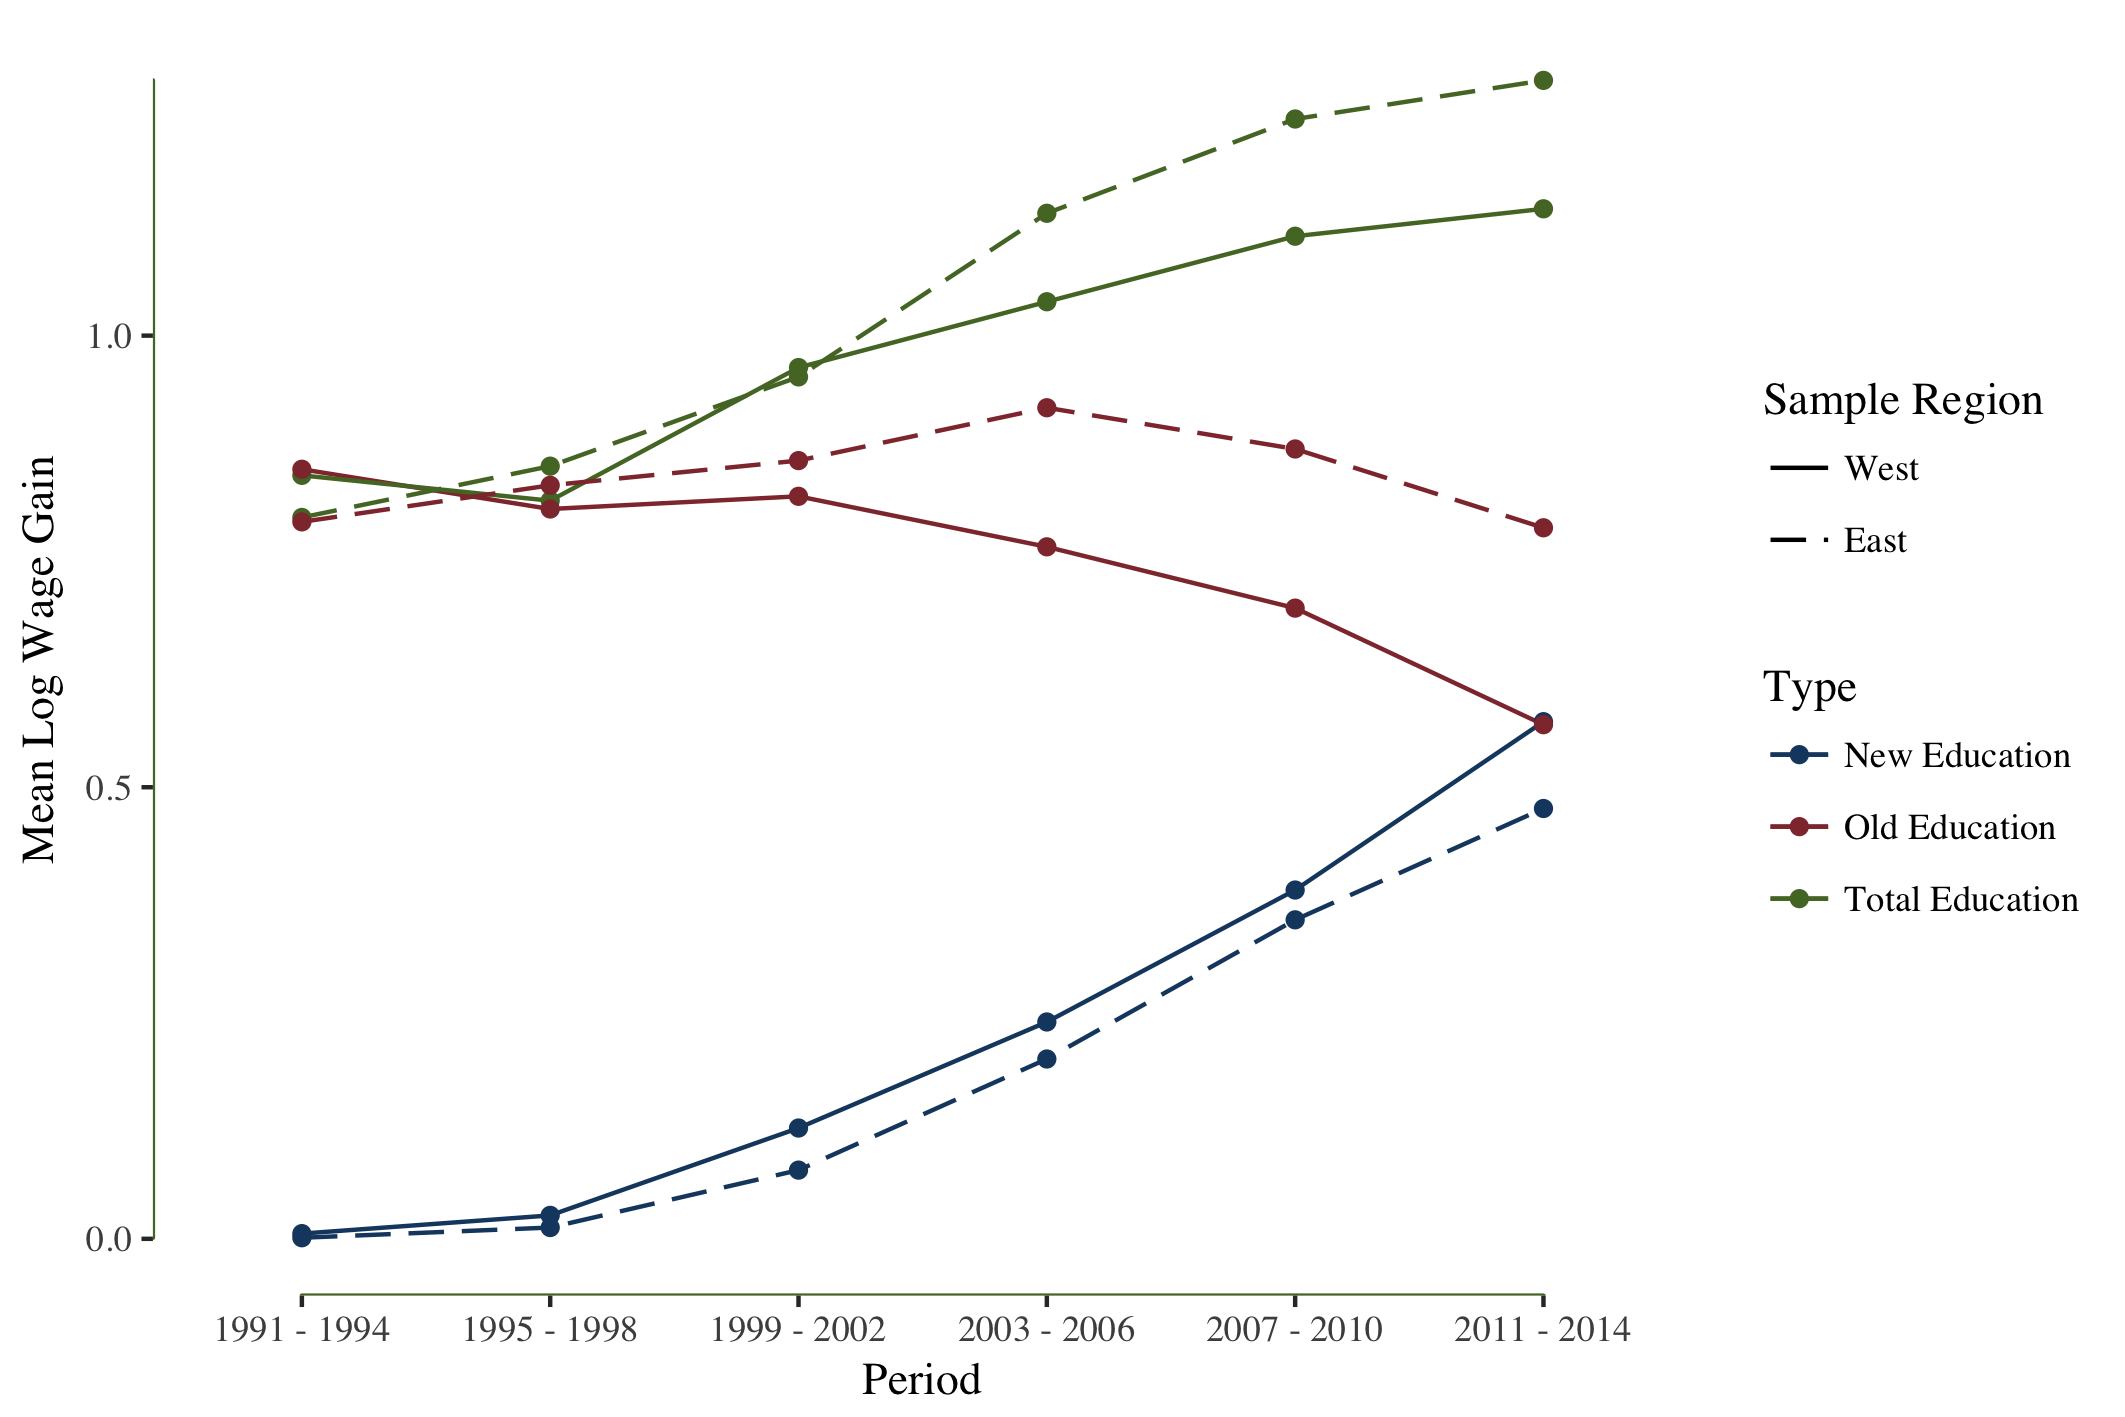
\includegraphics[width=\textwidth]{/Users/Christian/Statistik_Studium/EconProject/Code/Graphics/plotHumanCapitalEdu.png}
    \caption{Average Human Capital in Education}
    \label{fig:HumanCapitalEdu}
\end{figure}
\FloatBarrier

% tables (not mandatory)
\newgeometry{top=2.5cm,bottom=2.5cm,right=2.5cm,left=2.5cm}
\newpage
\section{Tables}
\FloatBarrier

\begin{table}
\begin{center}
\begin{small}
\begin{tabular}{l c c c c c c }
\hline
 & 1991 - 1994 & 1995 - 1998 & 1999 - 2002 & 2003 - 2006 & 2007 - 2010 & 2011 - 2014 \\
\hline
(Intercept)     & $6.8089^{***}$  & $6.8152^{***}$  & $6.6882^{***}$  & $6.6057^{***}$  & $6.4610^{***}$  & $6.4816^{***}$  \\
                & $(0.0199)$      & $(0.0223)$      & $(0.0239)$      & $(0.0257)$      & $(0.0258)$      & $(0.0249)$      \\
TotalEdu        & $0.0714^{***}$  & $0.0672^{***}$  & $0.0754^{***}$  & $0.0791^{***}$  & $0.0836^{***}$  & $0.0845^{***}$  \\
                & $(0.0014)$      & $(0.0014)$      & $(0.0015)$      & $(0.0016)$      & $(0.0016)$      & $(0.0016)$      \\
TotalExp        & $0.0332^{***}$  & $0.0388^{***}$  & $0.0408^{***}$  & $0.0459^{***}$  & $0.0466^{***}$  & $0.0409^{***}$  \\
                & $(0.0011)$      & $(0.0012)$      & $(0.0013)$      & $(0.0015)$      & $(0.0015)$      & $(0.0014)$      \\
TotalExpSquared & $-0.0006^{***}$ & $-0.0008^{***}$ & $-0.0008^{***}$ & $-0.0009^{***}$ & $-0.0009^{***}$ & $-0.0008^{***}$ \\
                & $(0.0000)$      & $(0.0000)$      & $(0.0000)$      & $(0.0000)$      & $(0.0000)$      & $(0.0000)$      \\
Tenure          & $0.0022^{***}$  & $0.0026^{***}$  & $0.0029^{***}$  & $0.0045^{***}$  & $0.0053^{***}$  & $0.0053^{***}$  \\
                & $(0.0005)$      & $(0.0005)$      & $(0.0006)$      & $(0.0007)$      & $(0.0007)$      & $(0.0007)$      \\
sex[2] weiblich & $-0.2701^{***}$ & $-0.2367^{***}$ & $-0.2321^{***}$ & $-0.2001^{***}$ & $-0.1846^{***}$ & $-0.2040^{***}$ \\
                & $(0.0078)$      & $(0.0085)$      & $(0.0090)$      & $(0.0096)$      & $(0.0099)$      & $(0.0095)$      \\
\hline
R$^2$           & 0.3823          & 0.3623          & 0.3821          & 0.3727          & 0.3974          & 0.3898          \\
Adj. R$^2$      & 0.3818          & 0.3618          & 0.3815          & 0.3721          & 0.3968          & 0.3892          \\
Num. obs.       & 10383           & 9016            & 8769            & 8483            & 7947            & 8488            \\
RMSE            & 0.3463          & 0.3530          & 0.3848          & 0.4107          & 0.4070          & 0.4096          \\
\hline
\multicolumn{7}{l}{\tiny{$^{***}p<0.001$, $^{**}p<0.01$, $^*p<0.05$}}
\end{tabular}
\end{small}
\caption{Model Coefficients for West German Data using Model 1}
\label{table:WestModelsTotal}
\end{center}
\end{table}


\begin{table}
\begin{center}
\begin{small}
\begin{tabular}{l c c c c c c }
\hline
 & 1991 - 1994 & 1995 - 1998 & 1999 - 2002 & 2003 - 2006 & 2007 - 2010 & 2011 - 2014 \\
\hline
(Intercept)     & $6.2025^{***}$  & $6.5169^{***}$  & $6.4577^{***}$  & $6.2844^{***}$  & $6.1174^{***}$  & $6.1040^{***}$  \\
                & $(0.0255)$      & $(0.0292)$      & $(0.0312)$      & $(0.0378)$      & $(0.0432)$      & $(0.0404)$      \\
TotalEdu        & $0.0640^{***}$  & $0.0676^{***}$  & $0.0737^{***}$  & $0.0862^{***}$  & $0.0929^{***}$  & $0.0957^{***}$  \\
                & $(0.0017)$      & $(0.0020)$      & $(0.0022)$      & $(0.0026)$      & $(0.0028)$      & $(0.0027)$      \\
TotalExp        & $0.0121^{***}$  & $0.0189^{***}$  & $0.0242^{***}$  & $0.0317^{***}$  & $0.0291^{***}$  & $0.0278^{***}$  \\
                & $(0.0014)$      & $(0.0016)$      & $(0.0016)$      & $(0.0020)$      & $(0.0024)$      & $(0.0022)$      \\
TotalExpSquared & $-0.0002^{***}$ & $-0.0004^{***}$ & $-0.0006^{***}$ & $-0.0007^{***}$ & $-0.0007^{***}$ & $-0.0007^{***}$ \\
                & $(0.0000)$      & $(0.0000)$      & $(0.0000)$      & $(0.0001)$      & $(0.0001)$      & $(0.0001)$      \\
Tenure          & $0.0017^{***}$  & $0.0075^{***}$  & $0.0084^{***}$  & $0.0094^{***}$  & $0.0114^{***}$  & $0.0132^{***}$  \\
                & $(0.0005)$      & $(0.0006)$      & $(0.0007)$      & $(0.0009)$      & $(0.0010)$      & $(0.0010)$      \\
sex[2] weiblich & $-0.1806^{***}$ & $-0.1304^{***}$ & $-0.1396^{***}$ & $-0.1747^{***}$ & $-0.1848^{***}$ & $-0.1661^{***}$ \\
                & $(0.0082)$      & $(0.0095)$      & $(0.0105)$      & $(0.0128)$      & $(0.0148)$      & $(0.0143)$      \\
\hline
R$^2$           & 0.3517          & 0.2423          & 0.2762          & 0.3056          & 0.2944          & 0.3474          \\
Adj. R$^2$      & 0.3510          & 0.2412          & 0.2750          & 0.3043          & 0.2930          & 0.3460          \\
Num. obs.       & 7242            & 5924            & 5155            & 4318            & 3927            & 3659            \\
RMSE            & 0.3430          & 0.3566          & 0.3688          & 0.4102          & 0.4459          & 0.4110          \\
\hline
\multicolumn{7}{l}{\tiny{$^{***}p<0.001$, $^{**}p<0.01$, $^*p<0.05$}}
\end{tabular}
\end{small}
\caption{Model Coefficients for East German Data using Model 1}
\label{table:EastModelsTotal}
\end{center}
\end{table}


\begin{table}
\begin{center}
\begin{small}
\begin{tabular}{l c c c c c c }
\hline
 & 1991 - 1994 & 1995 - 1998 & 1999 - 2002 & 2003 - 2006 & 2007 - 2010 & 2011 - 2014 \\
\hline
(Intercept)     & $6.7103^{***}$  & $6.6758^{***}$  & $6.6270^{***}$  & $6.5452^{***}$  & $6.4074^{***}$  & $6.3922^{***}$  \\
                & $(0.0241)$      & $(0.0296)$      & $(0.0282)$      & $(0.0314)$      & $(0.0319)$      & $(0.0295)$      \\
OldEdu          & $0.0727^{***}$  & $0.0691^{***}$  & $0.0756^{***}$  & $0.0781^{***}$  & $0.0816^{***}$  & $0.0809^{***}$  \\
                & $(0.0014)$      & $(0.0015)$      & $(0.0015)$      & $(0.0016)$      & $(0.0017)$      & $(0.0017)$      \\
NewEdu          & $0.0506^{***}$  & $0.0545^{***}$  & $0.0642^{***}$  & $0.0727^{***}$  & $0.0816^{***}$  & $0.0885^{***}$  \\
                & $(0.0067)$      & $(0.0039)$      & $(0.0026)$      & $(0.0024)$      & $(0.0022)$      & $(0.0019)$      \\
OldExp          & $0.0222^{***}$  & $0.0175^{***}$  & $0.0109^{***}$  & $0.0037$        & $0.0058^{*}$    & $0.0105^{**}$   \\
                & $(0.0011)$      & $(0.0013)$      & $(0.0017)$      & $(0.0023)$      & $(0.0027)$      & $(0.0034)$      \\
OldExpSquared   & $-0.0005^{***}$ & $-0.0004^{***}$ & $-0.0003^{***}$ & $-0.0002^{*}$   & $-0.0004^{**}$  & $-0.0008^{***}$ \\
                & $(0.0000)$      & $(0.0000)$      & $(0.0001)$      & $(0.0001)$      & $(0.0001)$      & $(0.0002)$      \\
NewExp          & $0.2374^{***}$  & $0.1156^{***}$  & $0.0839^{***}$  & $0.0803^{***}$  & $0.0690^{***}$  & $0.0561^{***}$  \\
                & $(0.0207)$      & $(0.0096)$      & $(0.0056)$      & $(0.0047)$      & $(0.0038)$      & $(0.0029)$      \\
NewExpSquared   & $-0.0272^{***}$ & $-0.0066^{***}$ & $-0.0036^{***}$ & $-0.0026^{***}$ & $-0.0019^{***}$ & $-0.0012^{***}$ \\
                & $(0.0044)$      & $(0.0011)$      & $(0.0004)$      & $(0.0003)$      & $(0.0002)$      & $(0.0001)$      \\
Tenure          & $0.0020^{***}$  & $0.0021^{***}$  & $0.0026^{***}$  & $0.0045^{***}$  & $0.0052^{***}$  & $0.0054^{***}$  \\
                & $(0.0005)$      & $(0.0005)$      & $(0.0006)$      & $(0.0007)$      & $(0.0007)$      & $(0.0007)$      \\
sex[2] weiblich & $-0.2651^{***}$ & $-0.2240^{***}$ & $-0.2155^{***}$ & $-0.1804^{***}$ & $-0.1686^{***}$ & $-0.1920^{***}$ \\
                & $(0.0077)$      & $(0.0085)$      & $(0.0090)$      & $(0.0096)$      & $(0.0100)$      & $(0.0096)$      \\
\hline
R$^2$           & 0.4005          & 0.3791          & 0.4000          & 0.3913          & 0.4082          & 0.3980          \\
Adj. R$^2$      & 0.3999          & 0.3784          & 0.3993          & 0.3905          & 0.4074          & 0.3973          \\
Num. obs.       & 10383           & 9016            & 8769            & 8483            & 7947            & 8488            \\
RMSE            & 0.3413          & 0.3483          & 0.3793          & 0.4046          & 0.4034          & 0.4069          \\
\hline
\multicolumn{7}{l}{\tiny{$^{***}p<0.001$, $^{**}p<0.01$, $^*p<0.05$}}
\end{tabular}
\end{small}
\caption{Model Coefficients for West German Data using Model 2}
\label{table:WestModelsOldNew}
\end{center}
\end{table}


\begin{table}
\begin{center}
\begin{small}
\begin{tabular}{l c c c c c c }
\hline
 & 1991 - 1994 & 1995 - 1998 & 1999 - 2002 & 2003 - 2006 & 2007 - 2010 & 2011 - 2014 \\
\hline
(Intercept)     & $6.1512^{***}$  & $6.4542^{***}$  & $6.4373^{***}$  & $6.2883^{***}$  & $6.0307^{***}$  & $6.0872^{***}$  \\
                & $(0.0304)$      & $(0.0384)$      & $(0.0391)$      & $(0.0490)$      & $(0.0552)$      & $(0.0492)$      \\
OldEdu          & $0.0639^{***}$  & $0.0674^{***}$  & $0.0734^{***}$  & $0.0855^{***}$  & $0.0899^{***}$  & $0.0933^{***}$  \\
                & $(0.0017)$      & $(0.0020)$      & $(0.0022)$      & $(0.0026)$      & $(0.0029)$      & $(0.0028)$      \\
NewEdu          & $0.0219$        & $0.0453^{***}$  & $0.0622^{***}$  & $0.0828^{***}$  & $0.0977^{***}$  & $0.0960^{***}$  \\
                & $(0.0121)$      & $(0.0064)$      & $(0.0041)$      & $(0.0039)$      & $(0.0037)$      & $(0.0032)$      \\
OldExp          & $0.0058^{***}$  & $-0.0035^{*}$   & $-0.0066^{**}$  & $-0.0014$       & $-0.0188^{***}$ & $-0.0191^{***}$ \\
                & $(0.0014)$      & $(0.0017)$      & $(0.0022)$      & $(0.0031)$      & $(0.0042)$      & $(0.0049)$      \\
OldExpSquared   & $-0.0001^{**}$  & $0.0001$        & $0.0000$        & $-0.0003^{**}$  & $0.0003$        & $0.0001$        \\
                & $(0.0000)$      & $(0.0001)$      & $(0.0001)$      & $(0.0001)$      & $(0.0002)$      & $(0.0003)$      \\
NewExp          & $0.1555^{***}$  & $0.0706^{***}$  & $0.0510^{***}$  & $0.0403^{***}$  & $0.0445^{***}$  & $0.0324^{***}$  \\
                & $(0.0284)$      & $(0.0131)$      & $(0.0082)$      & $(0.0075)$      & $(0.0066)$      & $(0.0049)$      \\
NewExpSquared   & $-0.0138^{*}$   & $-0.0009$       & $-0.0011$       & $-0.0006$       & $-0.0005$       & $-0.0005^{**}$  \\
                & $(0.0063)$      & $(0.0015)$      & $(0.0006)$      & $(0.0004)$      & $(0.0003)$      & $(0.0002)$      \\
Tenure          & $0.0010^{*}$    & $0.0053^{***}$  & $0.0061^{***}$  & $0.0072^{***}$  & $0.0079^{***}$  & $0.0108^{***}$  \\
                & $(0.0005)$      & $(0.0006)$      & $(0.0007)$      & $(0.0009)$      & $(0.0011)$      & $(0.0010)$      \\
sex[2] weiblich & $-0.1673^{***}$ & $-0.1027^{***}$ & $-0.1133^{***}$ & $-0.1504^{***}$ & $-0.1484^{***}$ & $-0.1424^{***}$ \\
                & $(0.0083)$      & $(0.0094)$      & $(0.0105)$      & $(0.0129)$      & $(0.0149)$      & $(0.0144)$      \\
\hline
R$^2$           & 0.3637          & 0.2808          & 0.3054          & 0.3228          & 0.3195          & 0.3630          \\
Adj. R$^2$      & 0.3628          & 0.2794          & 0.3039          & 0.3210          & 0.3176          & 0.3611          \\
Num. obs.       & 7242            & 5924            & 5155            & 4318            & 3927            & 3659            \\
RMSE            & 0.3399          & 0.3475          & 0.3614          & 0.4052          & 0.4381          & 0.4062          \\
\hline
\multicolumn{7}{l}{\tiny{$^{***}p<0.001$, $^{**}p<0.01$, $^*p<0.05$}}
\end{tabular}
\end{small}
\caption{Model Coefficients for East German Data using Model 2}
\label{table:EastModelsOldNew}
\end{center}
\end{table}





\end{document}
